\documentclass[14pt,a4paper]{extarticle}
% =============================================================
% preamble.tex — Shared LaTeX preamble for genetic/evolutionary reports
% Conforming to BSUIR STP 01-2024
% =============================================================

% Encoding and language
\usepackage[utf8]{inputenc}
\usepackage[T2A]{fontenc}
\usepackage[russian]{babel}

% Times New Roman font
\usepackage{tempora}

% Page geometry: STP 2.1.1
\usepackage{geometry}
\geometry{left=30mm, right=15mm, top=20mm, bottom=20mm}

% Line spacing: STP 2.1.1
\usepackage{setspace}
\singlespacing

% Allow TeX a bit more flexibility to avoid overflow
\pretolerance=1000
\tolerance=2000
\emergencystretch=3em

% Paragraph indent
\usepackage{indentfirst}
\setlength{\parindent}{1.25cm}

% Page numbers
\usepackage{fancyhdr}
\pagestyle{fancy}
\fancyhf{}
\fancyfoot[R]{\thepage}
\renewcommand{\headrulewidth}{0pt}
\fancypagestyle{plain}{%
  \fancyhf{}%
  \fancyfoot[R]{\thepage}%
  \renewcommand{\headrulewidth}{0pt}%
}

% Math
\usepackage{amsmath,amssymb}

% Graphics
\usepackage{graphicx}
\usepackage{float}
\usepackage{xcolor}

% Tables
\usepackage{booktabs}
\usepackage{tabularx}
\usepackage{multirow}
\usepackage{longtable}

% Captions
\usepackage{caption}
\captionsetup[figure]{
  labelsep=endash,
  justification=centering,
  font={normalsize},
  name=Рисунок
}
\captionsetup[table]{
  labelsep=endash,
  justification=raggedright,
  singlelinecheck=false,
  font={normalsize},
  name=Таблица
}

% Section formatting
\usepackage{titlesec}
\titleformat{\section}
  {\newpage\normalfont\fontsize{14}{18}\selectfont\bfseries}
  {\thesection}{0.5em}{\MakeUppercase}
\titlespacing*{\section}{1.25cm}{0pt}{14pt}

\titleformat{\subsection}
  {\normalfont\fontsize{14}{18}\selectfont\bfseries}
  {\thesubsection}{0.5em}{}
\titlespacing*{\subsection}{1.25cm}{14pt}{14pt}

\titleformat{\subsubsection}
  {\normalfont\fontsize{14}{18}\selectfont\bfseries}
  {\thesubsubsection}{0.5em}{}
\titlespacing*{\subsubsection}{1.25cm}{14pt}{14pt}

% Unnumbered sections
\newcommand{\sectioncenter}[1]{%
  \newpage
  \phantomsection
  \addcontentsline{toc}{section}{#1}
  \begin{center}
    \textbf{\MakeUppercase{#1}}
  \end{center}
  \vspace{14pt}
}

% Table of contents formatting
\usepackage{tocloft}
\renewcommand{\cftsecfont}{\normalfont}
\renewcommand{\cftsecpagefont}{\normalfont}
\renewcommand{\cftsubsecfont}{\normalfont}
\renewcommand{\cftsubsecpagefont}{\normalfont}
\renewcommand{\cftsecleader}{\cftdotfill{\cftdotsep}}
\renewcommand{\cftdotsep}{1}
\renewcommand{\contentsname}{\hfill\textbf{СОДЕРЖАНИЕ}\hfill}
\renewcommand{\cftaftertoctitle}{\hfill}

% Lists
\usepackage{enumitem}
\setlist[itemize]{noitemsep, topsep=0pt, leftmargin=1.25cm, label=--}
\setlist[enumerate]{noitemsep, topsep=0pt, leftmargin=1.25cm}

% Code listings
\usepackage{listings}
\usepackage{fancyvrb}
\lstset{
  basicstyle=\ttfamily\small,
  frame=single,
  breaklines=true,
  showstringspaces=false,
  inputencoding=utf8,
  extendedchars=true,
  literate={а}{{\cyra}}1 {б}{{\cyrb}}1 {в}{{\cyrv}}1 {г}{{\cyrg}}1
           {д}{{\cyrd}}1 {е}{{\cyre}}1 {ж}{{\cyrzh}}1 {з}{{\cyrz}}1
           {и}{{\cyri}}1 {й}{{\cyrishrt}}1 {к}{{\cyrk}}1 {л}{{\cyrl}}1
           {м}{{\cyrm}}1 {н}{{\cyrn}}1 {о}{{\cyro}}1 {п}{{\cyrp}}1
           {р}{{\cyrr}}1 {с}{{\cyrs}}1 {т}{{\cyrt}}1 {у}{{\cyru}}1
           {ф}{{\cyrf}}1 {х}{{\cyrh}}1 {ц}{{\cyrc}}1 {ч}{{\cyrch}}1
           {ш}{{\cyrsh}}1 {щ}{{\cyrshch}}1 {ъ}{{\cyrhrdsn}}1
           {ы}{{\cyrery}}1 {ь}{{\cyrsftsn}}1 {э}{{\cyrerev}}1
           {ю}{{\cyryu}}1 {я}{{\cyrya}}1
}

% Hyperlinks
\usepackage{hyperref}
\hypersetup{
  colorlinks=true,
  linkcolor=black,
  urlcolor=blue,
  citecolor=black,
}

% Number figures and tables within sections
\numberwithin{figure}{section}
\numberwithin{table}{section}
\numberwithin{equation}{section}

% Standard title page macro
\newcommand{\makegeclabtitle}[2]{%
  \begin{titlepage}
  \thispagestyle{empty}
  \begin{center}

  МИНИСТЕРСТВО ОБРАЗОВАНИЯ РЕСПУБЛИКИ БЕЛАРУСЬ

  \vspace{0.5em}

  Учреждение образования

  \vspace{0.5em}

  \textbf{<<Белорусский государственный университет информатики и радиоэлектроники>>}

  \vspace{2em}

  Факультет компьютерных систем и сетей

  \vspace{0.5em}

  Кафедра программного обеспечения информационных технологий

  \end{center}

  \vspace{3em}

  \begin{center}
  \textbf{ОТЧЕТ}

  \vspace{0.5em}

  по лабораторной работе №#1

  \vspace{0.5em}

  по дисциплине

  \vspace{0.5em}

  <<Генетические и эволюционные вычисления>>

  \vspace{0.5em}

  <<#2>>
  \end{center}

  \vspace{5em}

  \begin{flushright}
  \begin{minipage}{0.5\textwidth}
  \textbf{Выполнил:}\\
  Лебедевич Артем Владимирович\\
  магистрант группы 556301

  \vspace{0.6em}

  \textbf{Преподаватель:}\\
  Нестеренков Сергей Николаевич\\
  кандидат технических наук\\
  доцент кафедры ПОИТ
  \end{minipage}
  \end{flushright}

  \vfill

  \begin{center}
  Минск, 2026~г.
  \end{center}

  \end{titlepage}
}

\graphicspath{{figures/}}

\begin{document}

\makegeclabtitle{3}{Аппроксимация функции с помощью двухслойной нейронной сети}

\tableofcontents

\newpage

\section{Цель работы}

Изучить архитектуру двухслойной нейронной сети (многослойного персептрона), принципы её обучения методом обратного распространения ошибки (Backpropagation), а также исследовать точность аппроксимации нелинейной функции в зависимости от количества нейронов во внутреннем (скрытом) слое.

\section{Теоретические сведения}

\subsection{Двухслойная нейронная сеть}

Многослойный персептрон с одним скрытым и одним выходным слоем является универсальным аппроксиматором. Для скалярного входа $t$ выход скрытого слоя из $S$ нейронов вычисляется с нелинейной функцией активации <<гиперболический тангенс>> (\texttt{tansig}):
\begin{equation}
a_1 = \mathrm{tansig}(W_1 t + b_1), \qquad \mathrm{tansig}(z) = \frac{2}{1 + e^{-2z}} - 1 = \tanh z .
\end{equation}
Выходной слой с линейной функцией активации (\texttt{purelin}) линейно комбинирует полученные признаки:
\begin{equation}
y = \mathrm{purelin}(W_2 a_1 + b_2) = \sum_{i=1}^{S} w_{2,i} \tanh(w_{1,i} t + b_{1,i}) + b_2 .
\end{equation}
Таким образом, выход сети~--- сумма $S$ сдвинутых и масштабированных <<ступенек>> $\tanh$ плюс смещение; сеть 1--$S$--1 имеет $3S + 1$ настраиваемых параметров.

\subsection{Предобработка и инициализация (как в \texttt{newff})}

Функция \texttt{newff} по умолчанию нормирует входы и цели функцией \texttt{mapminmax} в диапазон $[-1, 1]$:
\begin{equation}
\tilde t = 2\,\frac{t - t_{\min}}{t_{\max} - t_{\min}} - 1,
\end{equation}
что удерживает аргументы $\tanh$ в области без насыщения. Веса скрытого слоя инициализируются по методу Нгуена~--- Уидроу (\texttt{initnw}): для одного входа $|w_{1,i}| = 0{,}7\,S$, а смещения $b_{1,i}$ равномерно распределены по $[-0{,}7S;\ 0{,}7S]$, так что активные области сигмоид с самого начала покрывают весь отрезок входа.

\subsection{Алгоритм обратного распространения ошибки}

Функция качества~--- среднеквадратичная ошибка
\begin{equation}
E = \frac{1}{N}\sum_{k=1}^{N} (\hat y_k - y_k)^2 .
\end{equation}
Градиенты вычисляются по правилу дифференцирования сложной функции, начиная с выхода:
\begin{equation}
\delta_2 = \frac{2}{N}(\hat y - y), \qquad \delta_1 = (\delta_2 W_2) \odot (1 - a_1^2),
\end{equation}
\begin{equation}
\frac{\partial E}{\partial W_2} = a_1^\top \delta_2, \quad \frac{\partial E}{\partial b_2} = \sum_k \delta_{2,k}, \quad
\frac{\partial E}{\partial W_1} = \tilde t^\top \delta_1, \quad \frac{\partial E}{\partial b_1} = \sum_k \delta_{1,k},
\end{equation}
где использовано $\tanh'(z) = 1 - \tanh^2 z$. Алгоритм \texttt{traingd} выполняет пакетный градиентный спуск
\begin{equation}
\theta^{(k+1)} = \theta^{(k)} - \eta\, \nabla_\theta E\bigl(\theta^{(k)}\bigr),
\end{equation}
где $\eta$~--- коэффициент обучения (\texttt{lr}). Для квадратичной аппроксимации функции ошибки спуск устойчив только при
\begin{equation}
\eta < \frac{2}{\lambda_{\max}},
\end{equation}
где $\lambda_{\max}$~--- наибольшее собственное число гессиана; скорость сходимости определяется числом обусловленности $\kappa = \lambda_{\max} / \lambda_{\min}$.

Обучение прекращается при выполнении любого из условий: $E \le$ \texttt{goal}, достигнуто \texttt{epochs} эпох, норма градиента меньше \texttt{min\_grad}. Параметр \texttt{show} задаёт период вывода промежуточных результатов.

\subsection{Ускоренные алгоритмы обучения}

Для сравнения рассмотрены алгоритмы MATLAB:
\begin{itemize}
\item \texttt{traingdx}~--- градиентный спуск с моментом ($mc = 0{,}9$) и адаптивным шагом: при уменьшении ошибки $\eta \leftarrow 1{,}05\,\eta$, при росте ошибки более чем в $1{,}04$ раза шаг отменяется и $\eta \leftarrow 0{,}7\,\eta$;
\item \texttt{trainlm}~--- метод Левенберга~--- Марквардта, использующий якобиан $J$ выходов сети по параметрам:
\begin{equation}
\Delta\theta = -\bigl(J^\top J + \mu I\bigr)^{-1} J^\top e,
\end{equation}
при малом $\mu$ шаг близок к шагу Гаусса~--- Ньютона, при большом~--- к короткому градиентному шагу.
\end{itemize}

\subsection{Теорема об универсальной аппроксимации}

Согласно теореме Цыбенко (1989) и её обобщению Хорником (1991), для любой непрерывной функции на компакте и любого $\varepsilon > 0$ существует сеть с одним скрытым слоем из конечного числа сигмоидальных нейронов и линейным выходом, приближающая функцию с точностью $\varepsilon$ в равномерной метрике.

\section{Ход работы}

\subsection{Исходные данные}

Вариант~3:
\begin{equation}
f(t) = (t + 1{,}3)\sin(0{,}5t + 1), \qquad t \in [-7;\ 7].
\end{equation}
Сформирован вектор $t = -7 : 0{,}1 : 7$ (141 точка) и вектор эталонных значений $y = f(t)$, $y \in [-8{,}11;\ 4{,}27]$. Функция имеет три экстремума: максимумы $f(-5{,}95) = 4{,}27$ и $f(2{,}18) = 3{,}02$ и минимум $f(-1{,}65) = -0{,}06$ (рисунок~\ref{fig:target}). Для оценки качества между узлами обучающей сетки использована контрольная сетка с шагом $0{,}01$ (1401 точка), не участвующая в обучении.

\subsection{Программная реализация}

Методические указания допускают Python или JavaScript вместо MATLAB. Выполнены две реализации без библиотек машинного обучения:
\begin{itemize}
\item \texttt{lab\_03.ipynb}~--- Python/NumPy: классы \texttt{MapMinMax} и \texttt{TwoLayerNet} (аналог \texttt{newff}, \texttt{sim}), функция \texttt{train} с алгоритмами \texttt{traingd}, \texttt{traingdm}, \texttt{traingdx}, \texttt{trainlm} и критериями останова MATLAB; протокол обучения выводится каждые \texttt{show} эпох в формате окна MATLAB. Корректность обратного распространения проверена сравнением с численным градиентом: относительная ошибка $4 \cdot 10^{-11}$;
\item \texttt{app/nn\_trainer.html}~--- интерактивное веб-приложение на JavaScript и Plotly.js (раздел~\ref{sec:app}).
\end{itemize}

Все интерактивные графики сохранены в каталоге \texttt{report/outputs/} в формате HTML (масштабирование, подсказки при наведении, анимация), статические копии~--- в \texttt{report/figures/}.

\subsection{Обучение по заданию с мультипликацией}

Сеть с $S = 10$ обучена алгоритмом \texttt{traingd} с параметрами \texttt{show = 50}, \texttt{lr = 0.05}, \texttt{epochs = 600}, \texttt{goal = 1e-2}. Протокол обучения:

\begin{verbatim}
TRAINGD, Epoch 0/600, MSE 144.86/0.01, Gradient 8.435/1e-05
TRAINGD, Epoch 50/600, MSE 0.79958/0.01, Gradient 0.0934/1e-05
TRAINGD, Epoch 100/600, MSE 0.46114/0.01, Gradient 0.03874/1e-05
TRAINGD, Epoch 200/600, MSE 0.27303/0.01, Gradient 0.02646/1e-05
TRAINGD, Epoch 300/600, MSE 0.16877/0.01, Gradient 0.02034/1e-05
TRAINGD, Epoch 400/600, MSE 0.10635/0.01, Gradient 0.01584/1e-05
TRAINGD, Epoch 500/600, MSE 0.068251/0.01, Gradient 0.01242/1e-05
TRAINGD, Epoch 600/600, MSE 0.044695/0.01, Gradient 0.009792/1e-05
\end{verbatim}

Обучение остановлено по лимиту эпох. Итог: MSE $= 0{,}045$ на обучающей и $0{,}044$ на контрольной сетке, $R^2 = 0{,}995$, максимальное отклонение $0{,}44$ при размахе функции $12{,}4$. Кривая аппроксимации перерисовывалась каждые 50 эпох синхронно с кривой ошибки (рисунки~\ref{fig:anim} и~\ref{fig:snapshots}): за первые 50 эпох сеть грубо повторяет форму функции (MSE падает со 145 до $0{,}8$), далее медленно <<дотягивает>> экстремумы.

\subsection{Серия экспериментов с разным числом нейронов}

Для $S \in \{1, 2, 5, 10, 20, 30\}$ выполнено по 10 запусков с разной начальной инициализацией при параметрах задания. Результаты приведены в таблице~\ref{tab:series} и на рисунках~\ref{fig:series}--\ref{fig:spread}.

\begin{table}[H]
\caption{Серия экспериментов по заданию (traingd, $\eta=0{,}05$, 600 эпох, 10 инициализаций)}
\label{tab:series}
\centering
\small
\begin{tabular}{cccccccc}
\toprule
$S$ & Параметров & MSE медиана & MSE лучшая & MSE худшая & MSE контроль & $R^2$ & Цель \\
\midrule
1 & 4 & 4.0830 & 3.2209 & 4.8133 & 4.0356 & 0.5335 & 0/10 \\
2 & 7 & 2.1762 & 2.1025 & 2.2680 & 2.1764 & 0.7535 & 0/10 \\
5 & 16 & 0.0484 & 0.0280 & 0.1664 & 0.0436 & 0.9948 & 0/10 \\
10 & 31 & 0.0493 & 0.0199 & 0.0840 & 0.0471 & 0.9944 & 0/10 \\
20 & 61 & 0.0670 & 0.0272 & 0.1045 & 0.0636 & 0.9923 & 0/10 \\
30 & 91 & 0.0958 & 0.0341 & 0.1208 & 0.0955 & 0.9890 & 0/10 \\
\bottomrule
\end{tabular}
\end{table}


\begin{itemize}
\item $S = 1$ и $S = 2$~--- явное недообучение: одна сигмоида даёт почти наклонную прямую, две~--- плавную ступеньку; экстремумы функции пропущены, $R^2 = 0{,}53$ и $0{,}75$.
\item $S = 5$ и $S = 10$~--- форма функции передана полностью, $R^2 \approx 0{,}995$; остаточная ошибка сосредоточена в экстремумах.
\item $S = 20$ и $S = 30$~--- медианная MSE выше ($0{,}067$ и $0{,}096$), на кривой видна мелкая рябь. Это недоученность, а не переобучение: ошибка на контрольной сетке равна ошибке на обучающей. Инициализация Нгуена~--- Уидроу делает сигмоиды тем круче, чем больше $S$ ($|w_1| = 0{,}7S$), и 600 малых шагов не успевают их согласовать.
\end{itemize}

Цель $10^{-2}$ за 600 эпох не достигнута ни в одном из 60 запусков: ограничивает не архитектура, а бюджет обучения.

\subsection{Доведение обучения до целевой ошибки}

Чтобы отделить возможности архитектуры от качества оптимизации, те же сети обучены: алгоритмом \texttt{traingd} без ограничения в 600 эпох (до 20\,000), а также алгоритмами \texttt{traingdx} и \texttt{trainlm} при прежнем лимите 600 эпох (таблица~\ref{tab:algos}, рисунок~\ref{fig:algos}).

\begin{table}[H]
\caption{Доведение обучения до целевой ошибки $10^{-2}$ (медиана по 10 инициализациям)}
\label{tab:algos}
\centering
\small
\begin{tabular}{lccccc}
\toprule
Алгоритм & $S$ & MSE медиана & MSE контроль & Эпох & Цель \\
\midrule
traingd ($\le$20000 эп.) & 1 & 1.5527 & 1.5578 & 20000 & 0/10 \\
traingd ($\le$20000 эп.) & 2 & 0.8646 & 0.8664 & 20000 & 0/10 \\
traingd ($\le$20000 эп.) & 5 & 0.0100 & 0.0090 & 3673 & 10/10 \\
traingd ($\le$20000 эп.) & 10 & 0.0100 & 0.0090 & 2360 & 10/10 \\
traingd ($\le$20000 эп.) & 20 & 0.0100 & 0.0090 & 2618 & 10/10 \\
traingd ($\le$20000 эп.) & 30 & 0.0100 & 0.0097 & 3961 & 10/10 \\
traingdx & 1 & 1.5105 & 1.5153 & 600 & 0/10 \\
traingdx & 2 & 0.7761 & 0.7779 & 600 & 0/10 \\
traingdx & 5 & 0.0100 & 0.0089 & 145 & 10/10 \\
traingdx & 10 & 0.0099 & 0.0089 & 117 & 10/10 \\
traingdx & 20 & 0.0099 & 0.0089 & 196 & 10/10 \\
traingdx & 30 & 0.0100 & 0.0097 & 386 & 10/10 \\
trainlm & 1 & 1.5039 & 1.5076 & 25 & 0/10 \\
trainlm & 2 & 0.6751 & 0.6770 & 66 & 0/10 \\
trainlm & 5 & 0.0071 & 0.0067 & 5 & 10/10 \\
trainlm & 10 & 0.0030 & 0.0030 & 3 & 10/10 \\
trainlm & 20 & 0.0027 & 0.0026 & 1 & 10/10 \\
trainlm & 30 & 9.1e-4 & 8.6e-4 & 1 & 10/10 \\
\bottomrule
\end{tabular}
\end{table}


При $S \ge 5$ цель достигается во всех запусках: \texttt{traingd} требуется 2360--3960 эпох, \texttt{traingdx}~--- 117--386, \texttt{trainlm}~--- 1--5 эпох. Сети с $S = 1$ и $S = 2$ не достигают цели ни одним алгоритмом.

Предельная точность при данном $S$ определена обучением \texttt{trainlm} практически до сходимости (\texttt{goal = 1e-10}, до 500 эпох, лучший из 10 запусков), таблица~\ref{tab:capacity} и рисунки~\ref{fig:capacity}--\ref{fig:contrib}.

\begin{table}[H]
\caption{Предельная точность сети с $S$ нейронами (trainlm, лучший из 10 запусков)}
\label{tab:capacity}
\centering
\small
\begin{tabular}{cccc}
\toprule
$S$ & MSE обучение & MSE контроль & max$|e|$ \\
\midrule
1 & 1.5e+00 & 1.5e+00 & 2.2e+00 \\
2 & 6.8e-01 & 6.8e-01 & 1.6e+00 \\
3 & 9.3e-05 & 8.5e-05 & 4.4e-02 \\
4 & 8.7e-06 & 8.3e-06 & 7.8e-03 \\
5 & 7.3e-09 & 6.9e-09 & 2.9e-04 \\
10 & 2.5e-09 & 2.2e-09 & 2.4e-04 \\
20 & 9.7e-10 & 1.0e-09 & 1.4e-04 \\
30 & 3.4e-10 & 4.7e-10 & 1.7e-04 \\
\bottomrule
\end{tabular}
\end{table}


Минимальное число нейронов, при котором цель $10^{-2}$ достижима, равно трём~--- по одному на каждый изгиб функции. Уже при $S = 5$ ошибка снижается до $\sim 10^{-8}$, дальнейшее увеличение $S$ практически ничего не даёт. Ошибка на контрольной сетке совпадает с ошибкой на обучающей: на точных данных с шагом $0{,}1$ переобучения нет.

\subsection{Влияние коэффициента обучения}

Для $S = 10$ исследованы значения $\eta$ из допустимого диапазона $[0{,}01;\ 0{,}5]$ (таблица~\ref{tab:lr}, рисунок~\ref{fig:lr}).

\begin{table}[H]
\caption{Влияние коэффициента обучения (traingd, $S=10$, 600 эпох, 10 инициализаций)}
\label{tab:lr}
\centering
\small
\begin{tabular}{ccccc}
\toprule
$\eta$ & MSE медиана & Цель достигнута & Эпох до цели & Расходимость \\
\midrule
0.01 & 0.2342 & 0/10 & — & 0/10 \\
0.05 & 0.0493 & 0/10 & — & 0/10 \\
0.1 & 0.0262 & 2/10 & 477 & 0/10 \\
0.2 & 0.0100 & 8/10 & 332 & 0/10 \\
0.25 & --- & 0/10 & — & 10/10 \\
0.3 & --- & 0/10 & — & 10/10 \\
0.5 & --- & 0/10 & — & 10/10 \\
\bottomrule
\end{tabular}
\end{table}


До $\eta = 0{,}2$ рост шага ускоряет сходимость, при $\eta \ge 0{,}25$ обучение расходится во всех запусках. Оценка гессиана приближением Гаусса~--- Ньютона $H \approx \frac{2}{N} J^\top J$ даёт $\lambda_{\max} \approx 10{,}5$, т.е. критический шаг $2/\lambda_{\max} \approx 0{,}19$, что согласуется с экспериментом. Число обусловленности $\kappa \sim 10^{11}$--$10^{12}$: поверхность ошибки~--- узкий <<овраг>>, поэтому допустимый шаг ограничен крутыми направлениями, а вдоль пологих спуск идёт очень медленно. Именно это объясняет тысячи эпох \texttt{traingd} и выигрыш алгоритмов, учитывающих кривизну.

\subsection{Недообучение и переобучение}

На точной функции с плотной сеткой переобучение не проявляется, поэтому к обучающим значениям добавлен шум $\mathcal N(0;\ 0{,}7^2)$, а качество оценивается по истинной функции на контрольной сетке. Сети обучены \texttt{trainlm} до минимума ошибки (1000 эпох). Дополнительно для $S = 30$ применён ранний останов: разбиение 70/15/15\,\% и остановка после 6 последовательных ростов ошибки на валидации (как \texttt{dividerand} и \texttt{max\_fail} в MATLAB). Результаты~--- в таблице~\ref{tab:noise} и на рисунках~\ref{fig:overfit}--\ref{fig:bv}.

\begin{table}[H]
\caption{Недообучение и переобучение на зашумлённых данных ($\sigma = 0{,}7$, trainlm)}
\label{tab:noise}
\centering
\small
\begin{tabular}{ccc}
\toprule
$S$ & MSE на шумных точках & MSE относительно $f(t)$ \\
\midrule
1 & 1.835 & 1.512 \\
2 & 1.041 & 0.684 \\
3 & 0.531 & 0.060 \\
5 & 0.487 & 0.066 \\
8 & 0.409 & 0.135 \\
10 & 0.360 & 0.231 \\
15 & 0.299 & 0.266 \\
20 & 0.249 & 0.350 \\
30 & 0.170 & 4.062 \\
30 + ранний останов & 0.277 & 0.374 \\
\bottomrule
\end{tabular}
\end{table}


Ошибка на обучающих точках монотонно уменьшается с ростом $S$, а ошибка относительно истинной функции имеет U-образную форму с минимумом при $S = 3$ ($0{,}060$). При $S = 30$ ошибка на обучении ($0{,}17$) ниже дисперсии шума ($0{,}49$)~--- сеть запоминает шум; кривая проходит через обучающие точки и даёт узкий выброс от $-23$ до $+32$ около $t \approx 0{,}1$, ошибка относительно истинной функции~--- $4{,}06$. Ранний останов уменьшает её до $0{,}37$, т.е. в 11 раз.

\subsection{Интерактивное приложение}
\label{sec:app}

Приложение \texttt{app/nn\_trainer.html} (рисунок~\ref{fig:app}) реализует требования раздела~3 методических указаний:
\begin{itemize}
\item ползунок числа нейронов скрытого слоя от 1 до 30;
\item ручной ввод коэффициента обучения $\eta \in [0{,}01;\ 0{,}5]$ и целевой ошибки \texttt{goal} $\in [10^{-4};\ 10^{-1}]$ с проверкой диапазона, а также \texttt{epochs}, \texttt{show}, выбор алгоритма и начальной инициализации;
\item координатная плоскость с точками исходной функции и непрерывной кривой аппроксимации, которая перерисовывается каждые \texttt{show} эпох; бледный <<след>> прошлых положений кривой показывает процесс её изгибания;
\item синхронный график ошибки, выстраиваемый точка за точкой, с линией \texttt{goal} и отметками перерисовок;
\item ползунок <<Задержка (мс)>> и кнопки <<Старт>>, <<Пауза>>, <<Сброс>> (также клавиши <<Пробел>> и <<R>>);
\item дополнительно: выбор любого из 14 вариантов, график вкладов отдельных нейронов, кнопка серийного эксперимента для $S = 1, 2, 5, 10, 20, 30$ с таблицей результатов.
\end{itemize}

\section{Результаты}

\begin{enumerate}
\item Реализована двухслойная сеть \texttt{tansig}--\texttt{purelin} с обучением обратным распространением ошибки; корректность градиентов подтверждена численной проверкой.
\item По параметрам задания (\texttt{traingd}, $\eta = 0{,}05$, 600 эпох) сеть с $S = 10$ аппроксимирует функцию с MSE $= 0{,}045$ и $R^2 = 0{,}995$; цель $10^{-2}$ за 600 эпох не достигается.
\item Точность аппроксимации определяется числом нейронов до $S \approx 5$: $S = 1, 2$~--- недообучение (MSE не ниже $1{,}5$ и $0{,}68$ при любом обучении), $S \ge 3$~--- цель достижима, $S \ge 5$~--- MSE $\sim 10^{-8}$.
\item При фиксированном бюджете 600 эпох большие сети ($S = 20, 30$) обучаются хуже средних из-за более сложной оптимизации.
\item Ускоренные алгоритмы достигают цели на порядки быстрее: \texttt{traingdx}~--- за сотни эпох, \texttt{trainlm}~--- за единицы.
\item Граница устойчивости \texttt{traingd} $\eta \approx 0{,}2$ совпадает с теоретической $2/\lambda_{\max} \approx 0{,}19$.
\item На зашумлённых данных избыточная сеть ($S = 30$) переобучается; оптимальное $S = 3$, ранний останов снижает ошибку избыточной сети в 11 раз.
\end{enumerate}

\section{Иллюстрации результатов}

Ниже приведены основные визуализации, полученные в ходе выполнения лабораторной работы. Интерактивные версии графиков находятся в каталоге \texttt{outputs/}.

\begin{figure}[H]
\centering
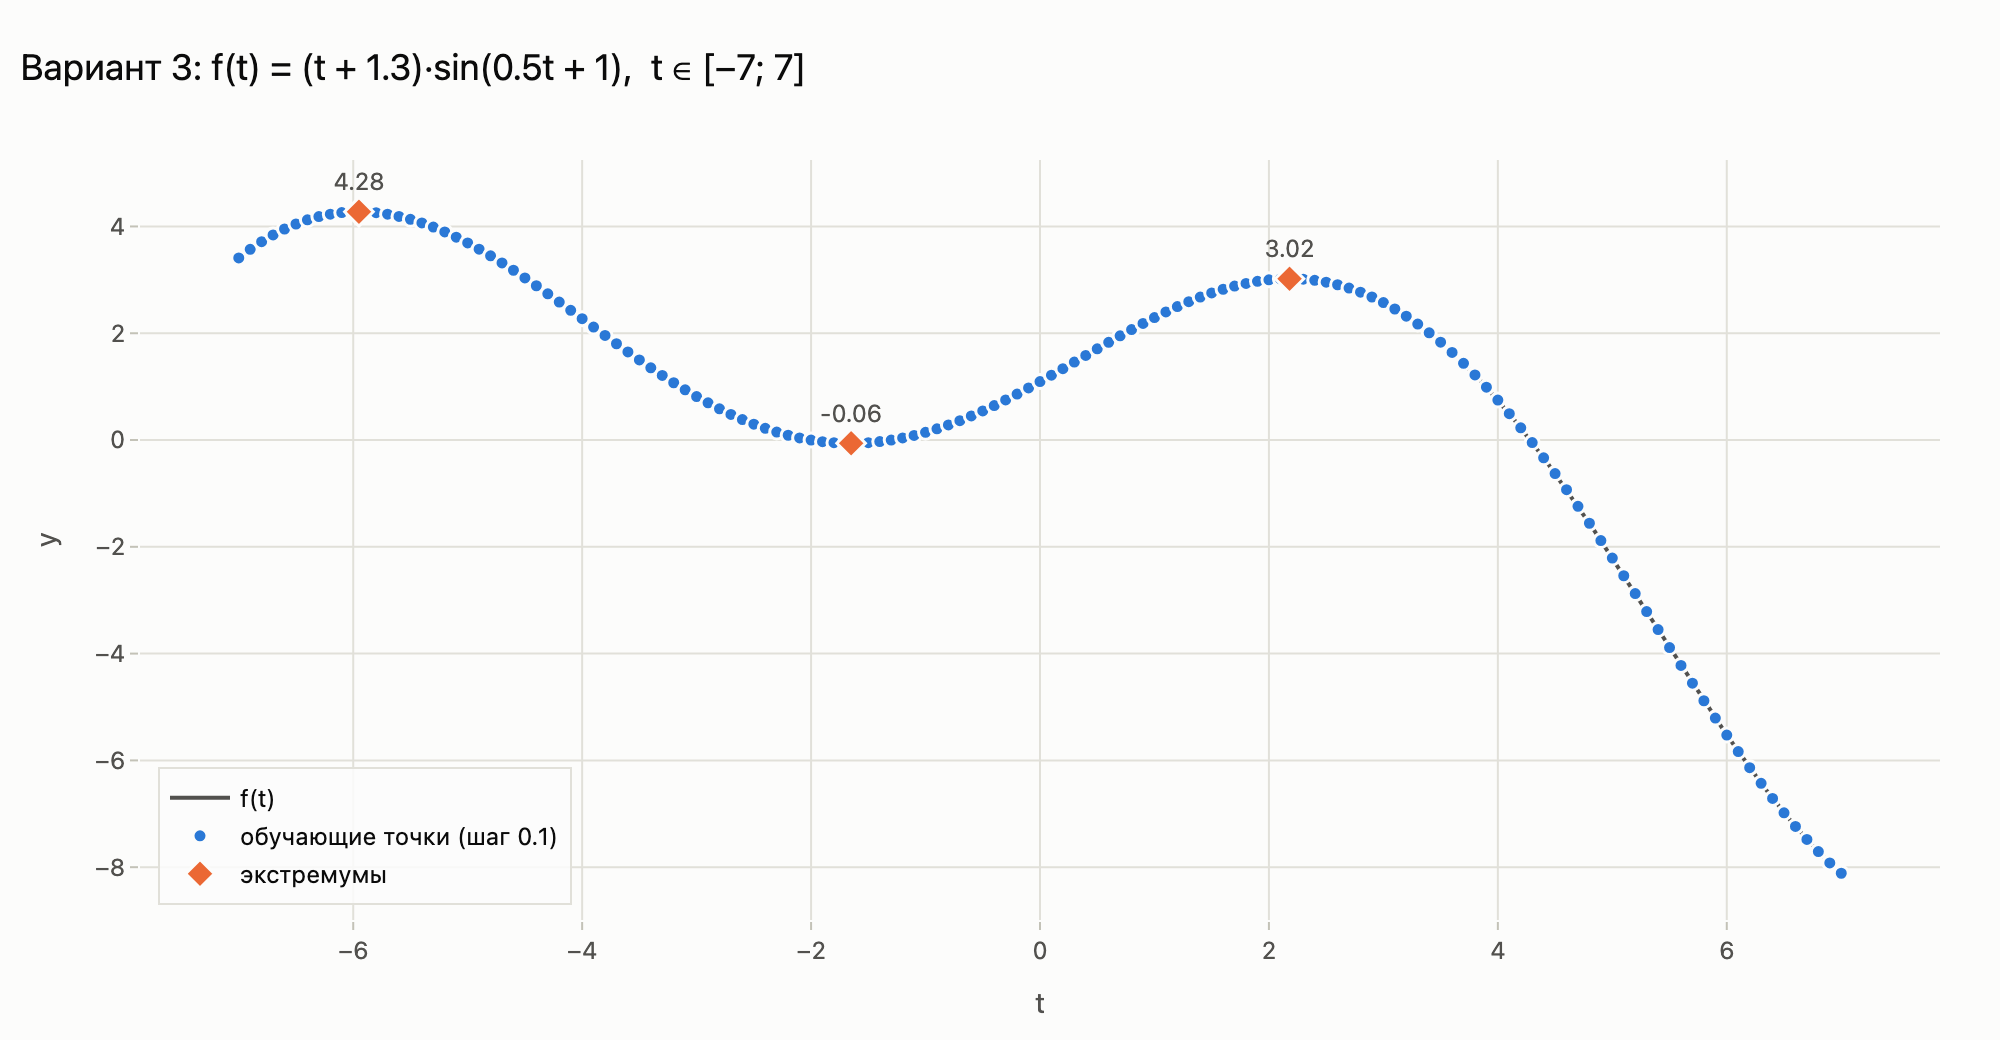
\includegraphics[width=\textwidth]{01_target_function.png}
\caption{Функция варианта~3 и обучающие точки с шагом 0,1.}
\label{fig:target}
\end{figure}

\begin{figure}[H]
\centering
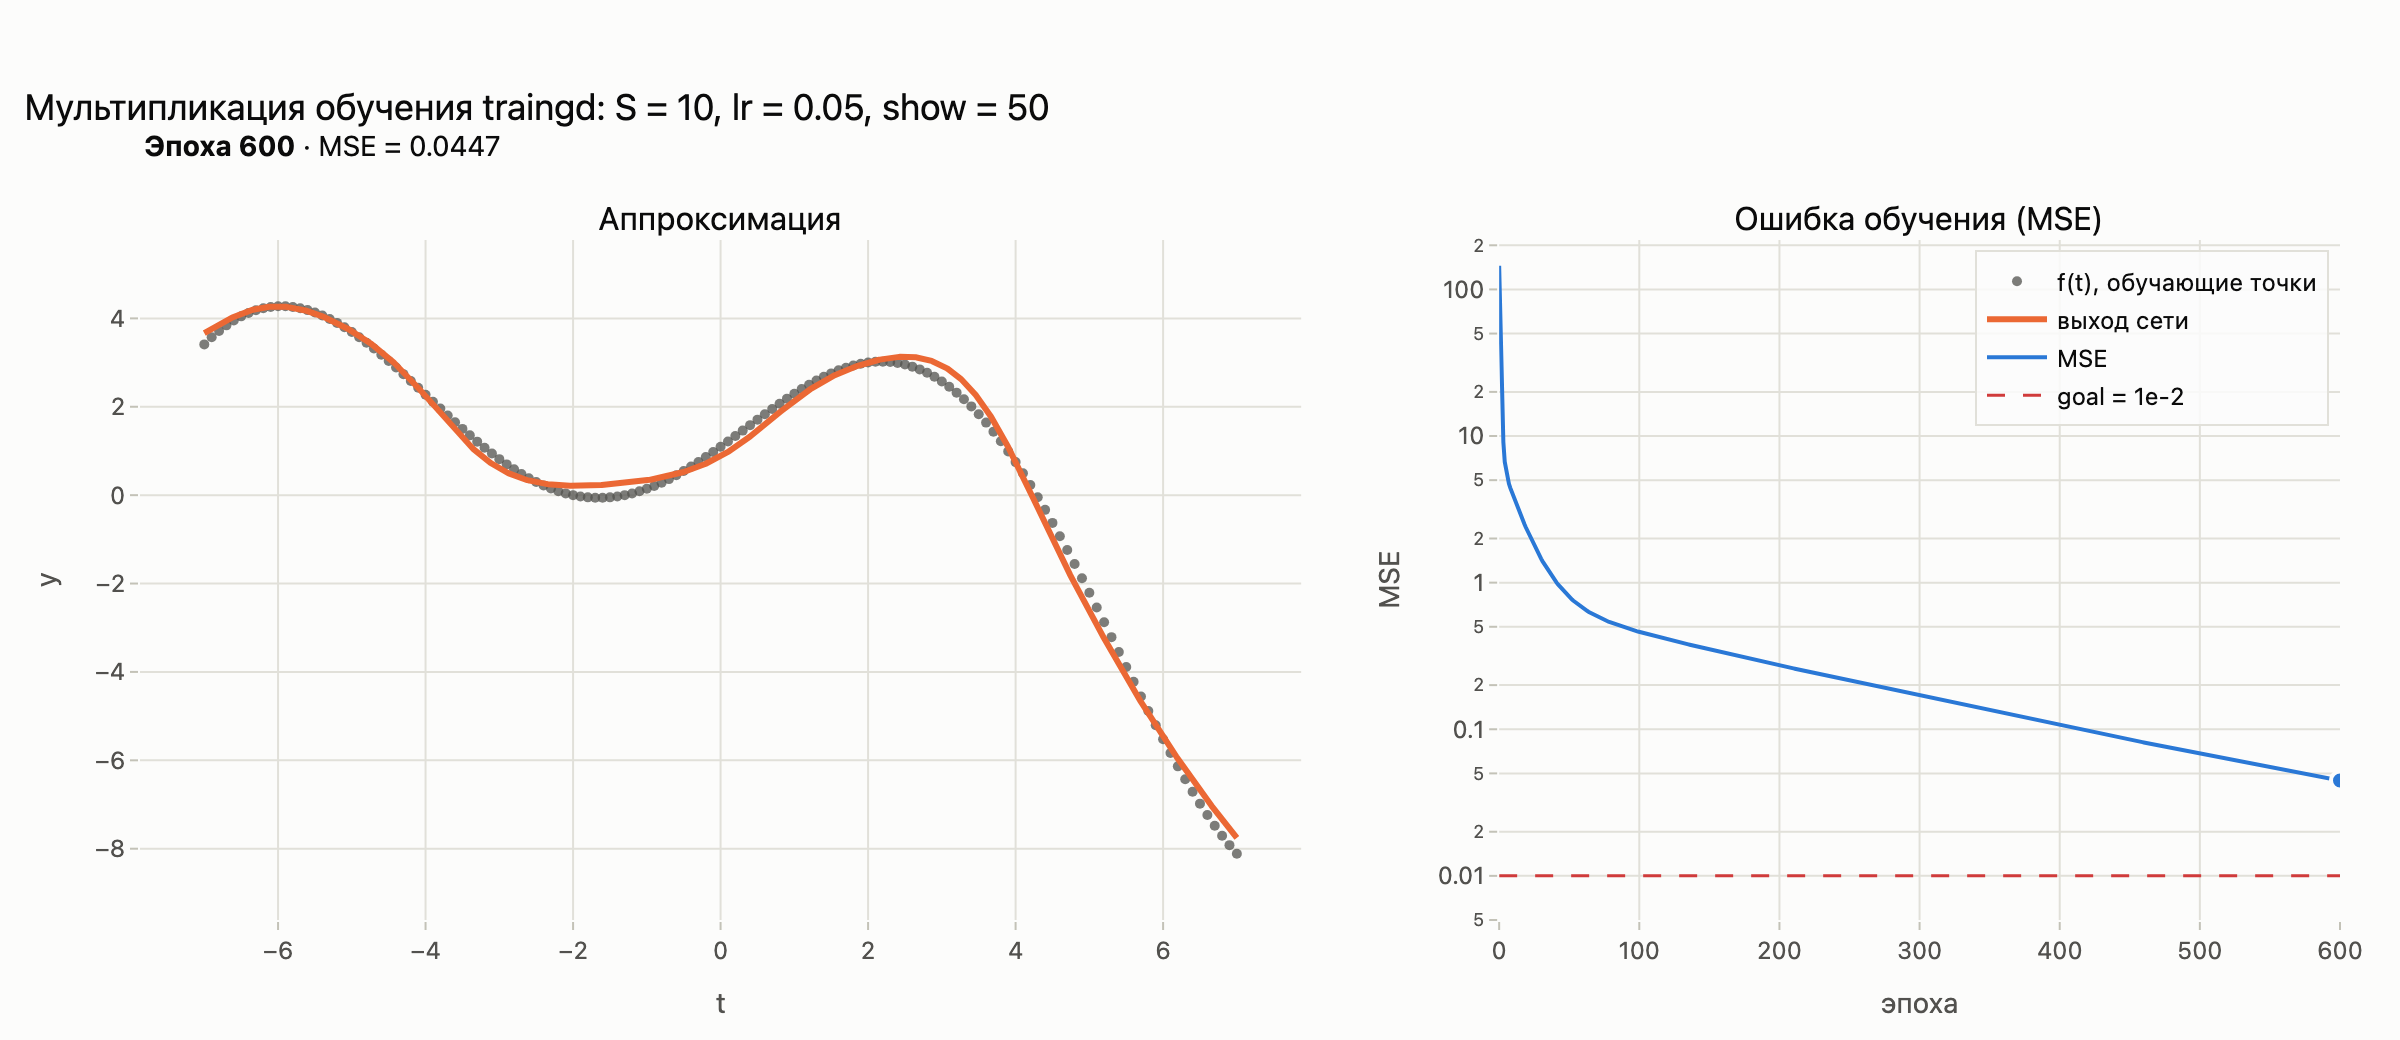
\includegraphics[width=\textwidth]{02_training_animation.png}
\caption{Мультипликация обучения traingd ($S = 10$): финальный кадр. Интерактивная версия с кнопками <<Старт>>, <<Пауза>>, <<Сброс>>~--- \texttt{outputs/02\_training\_animation.html}.}
\label{fig:anim}
\end{figure}

\begin{figure}[H]
\centering
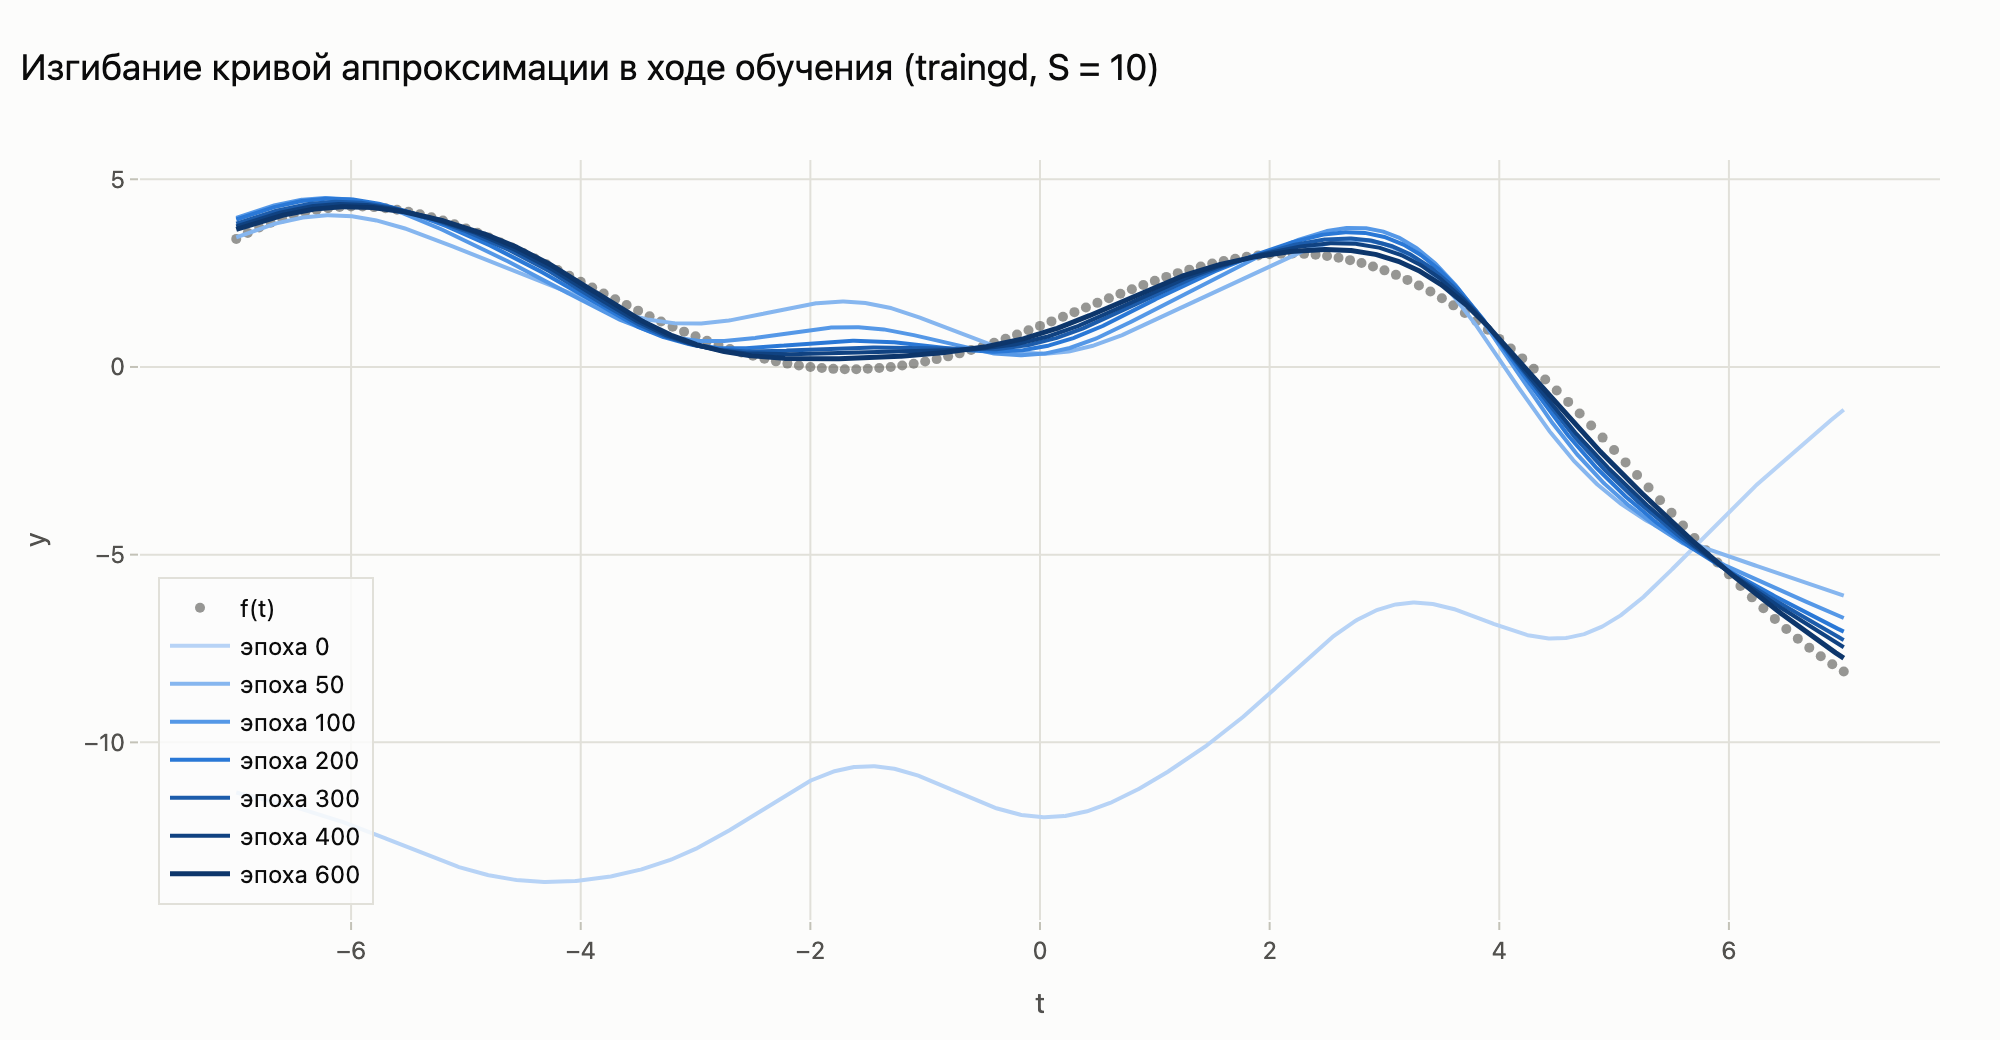
\includegraphics[width=\textwidth]{03_training_snapshots.png}
\caption{Изгибание кривой аппроксимации в ходе обучения traingd ($S = 10$).}
\label{fig:snapshots}
\end{figure}

\begin{figure}[H]
\centering
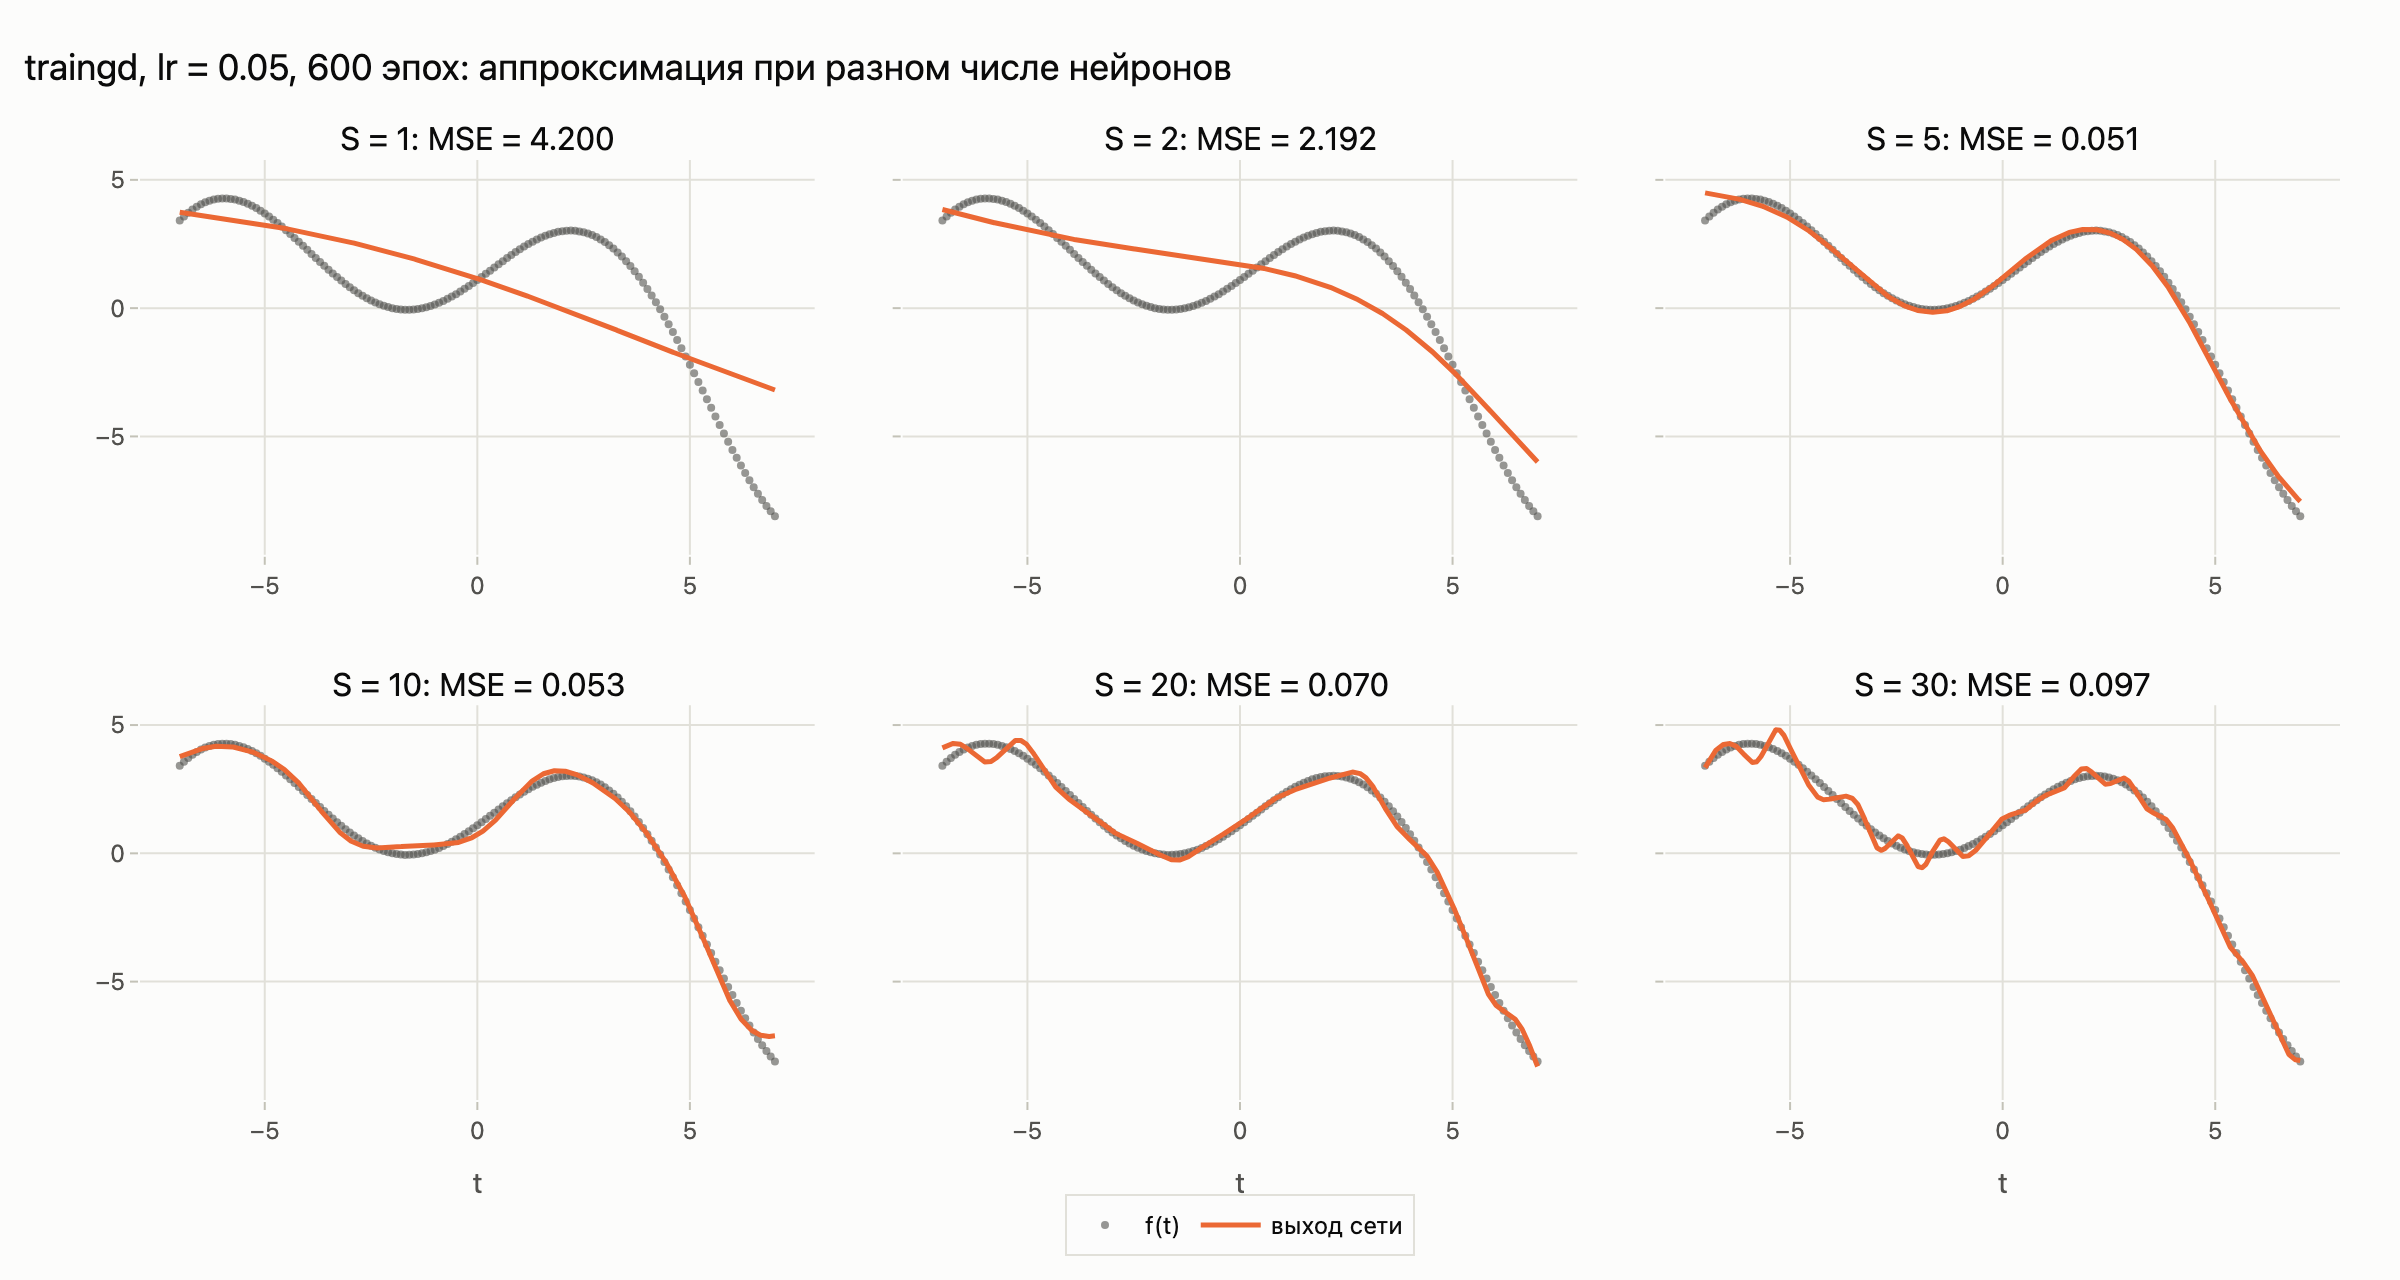
\includegraphics[width=\textwidth]{04_series_approximations.png}
\caption{Аппроксимация при $S = 1, 2, 5, 10, 20, 30$ (traingd, $\eta = 0{,}05$, 600 эпох, типичный запуск).}
\label{fig:series}
\end{figure}

\begin{figure}[H]
\centering
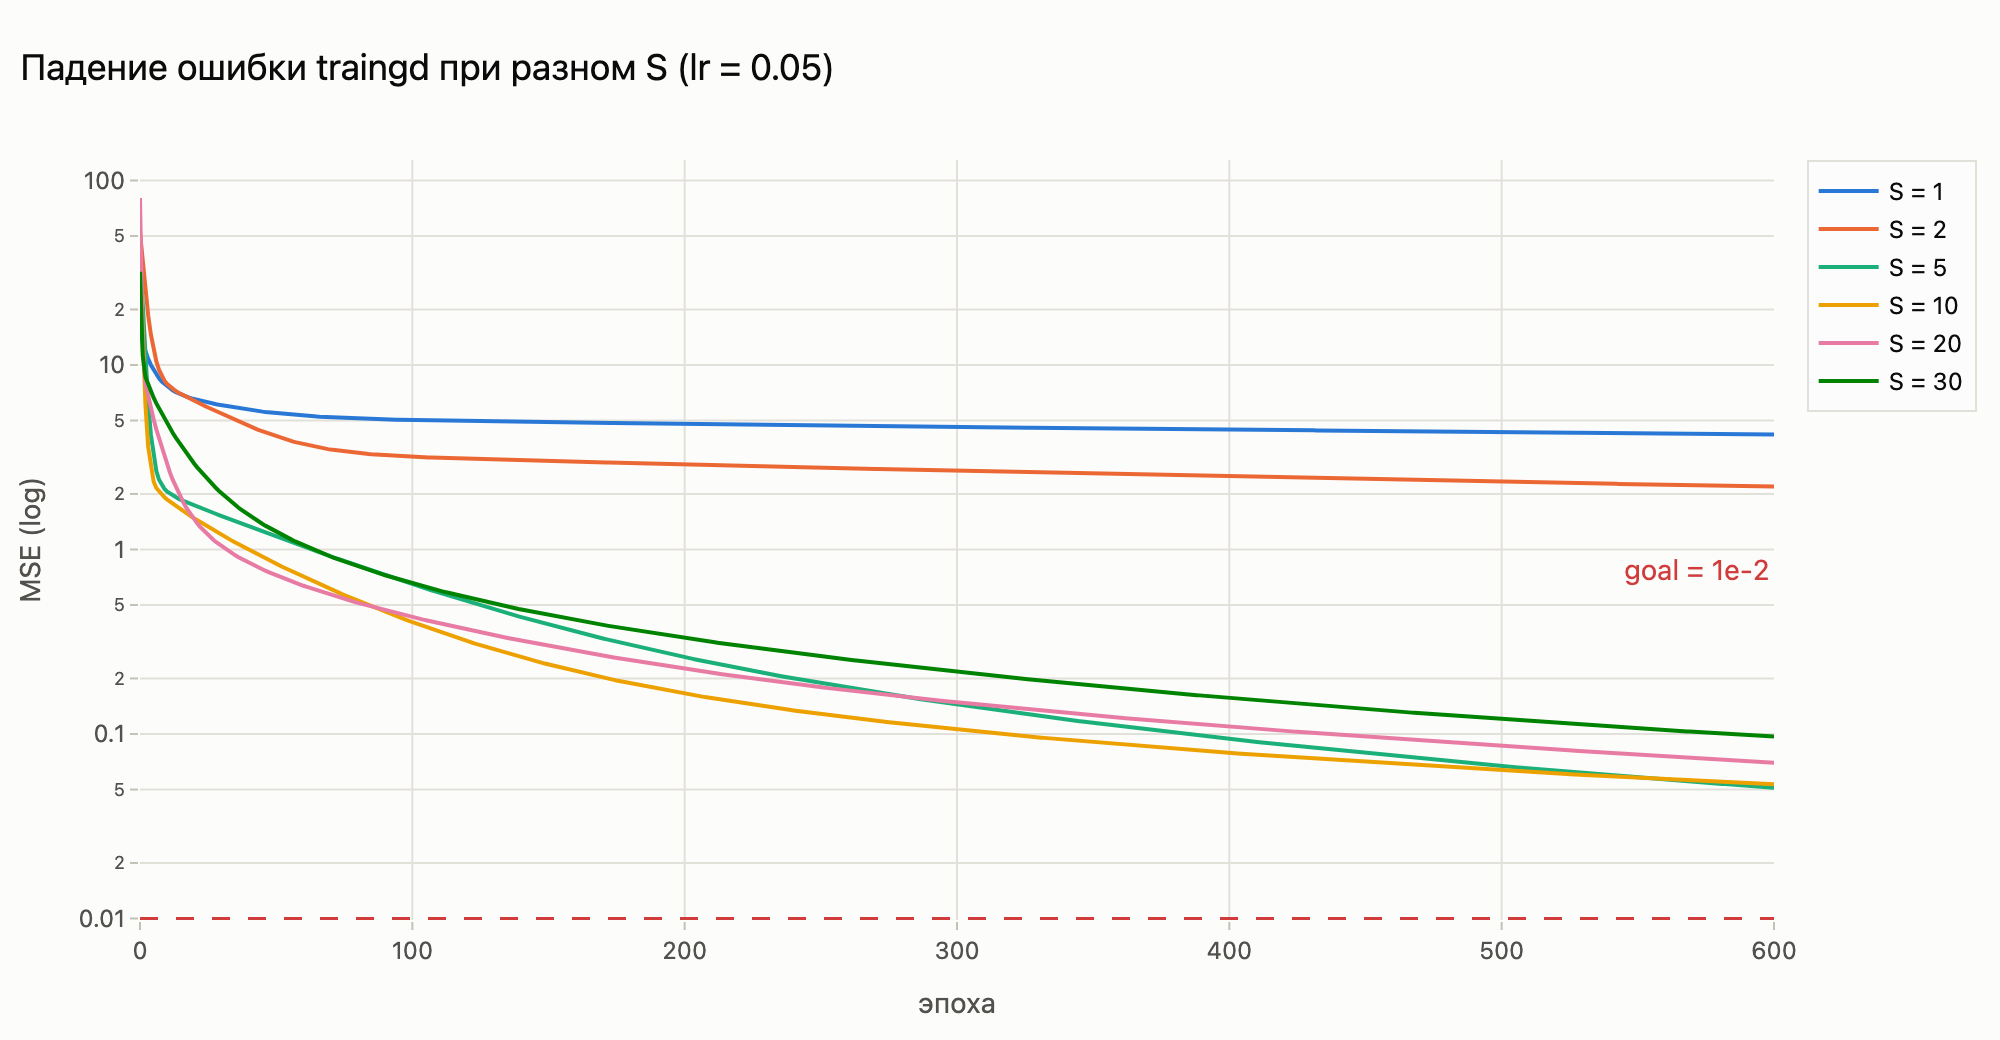
\includegraphics[width=\textwidth]{05_series_performance.png}
\caption{Кривые ошибки traingd при разном числе нейронов.}
\label{fig:seriesperf}
\end{figure}

\begin{figure}[H]
\centering
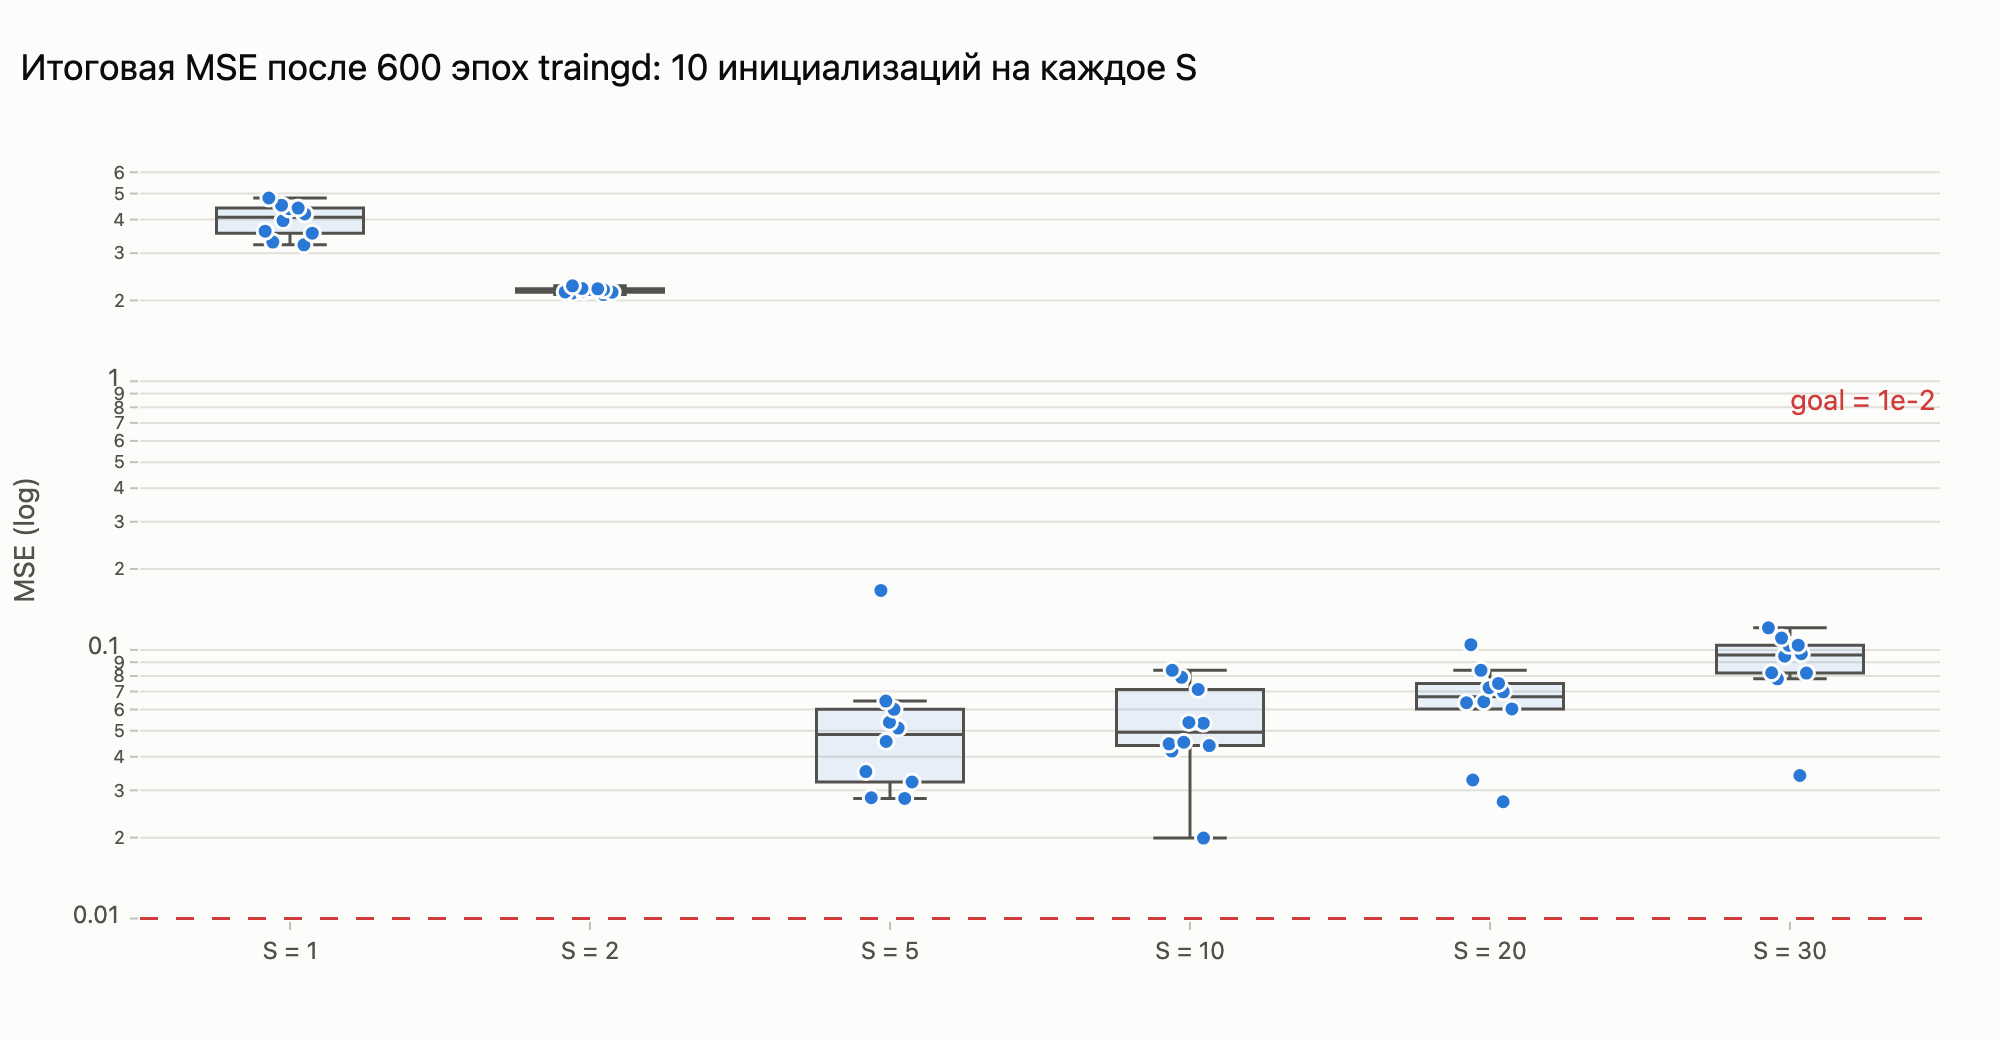
\includegraphics[width=\textwidth]{06_series_mse_spread.png}
\caption{Разброс итоговой MSE по 10 инициализациям.}
\label{fig:spread}
\end{figure}

\begin{figure}[H]
\centering
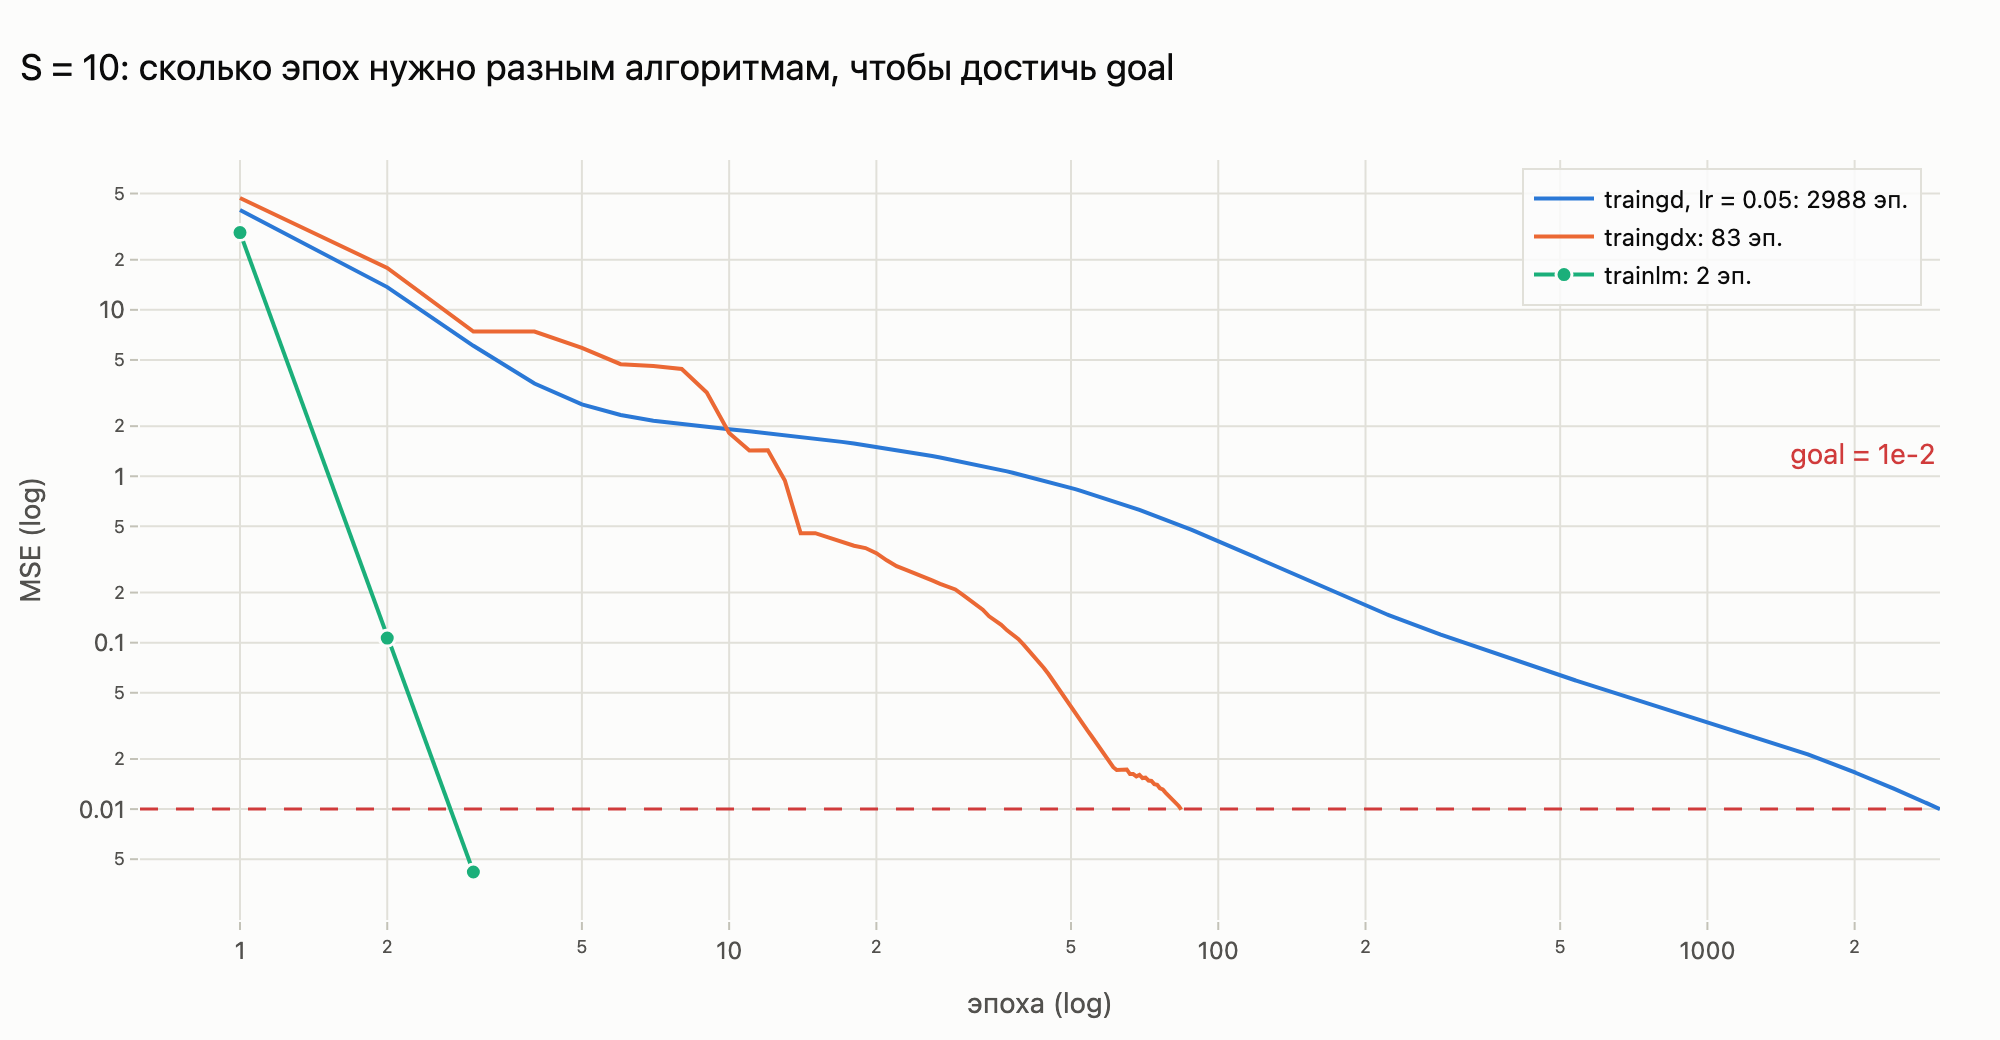
\includegraphics[width=\textwidth]{07_algorithms_convergence.png}
\caption{Скорость сходимости traingd, traingdx и trainlm при $S = 10$.}
\label{fig:algos}
\end{figure}

\begin{figure}[H]
\centering
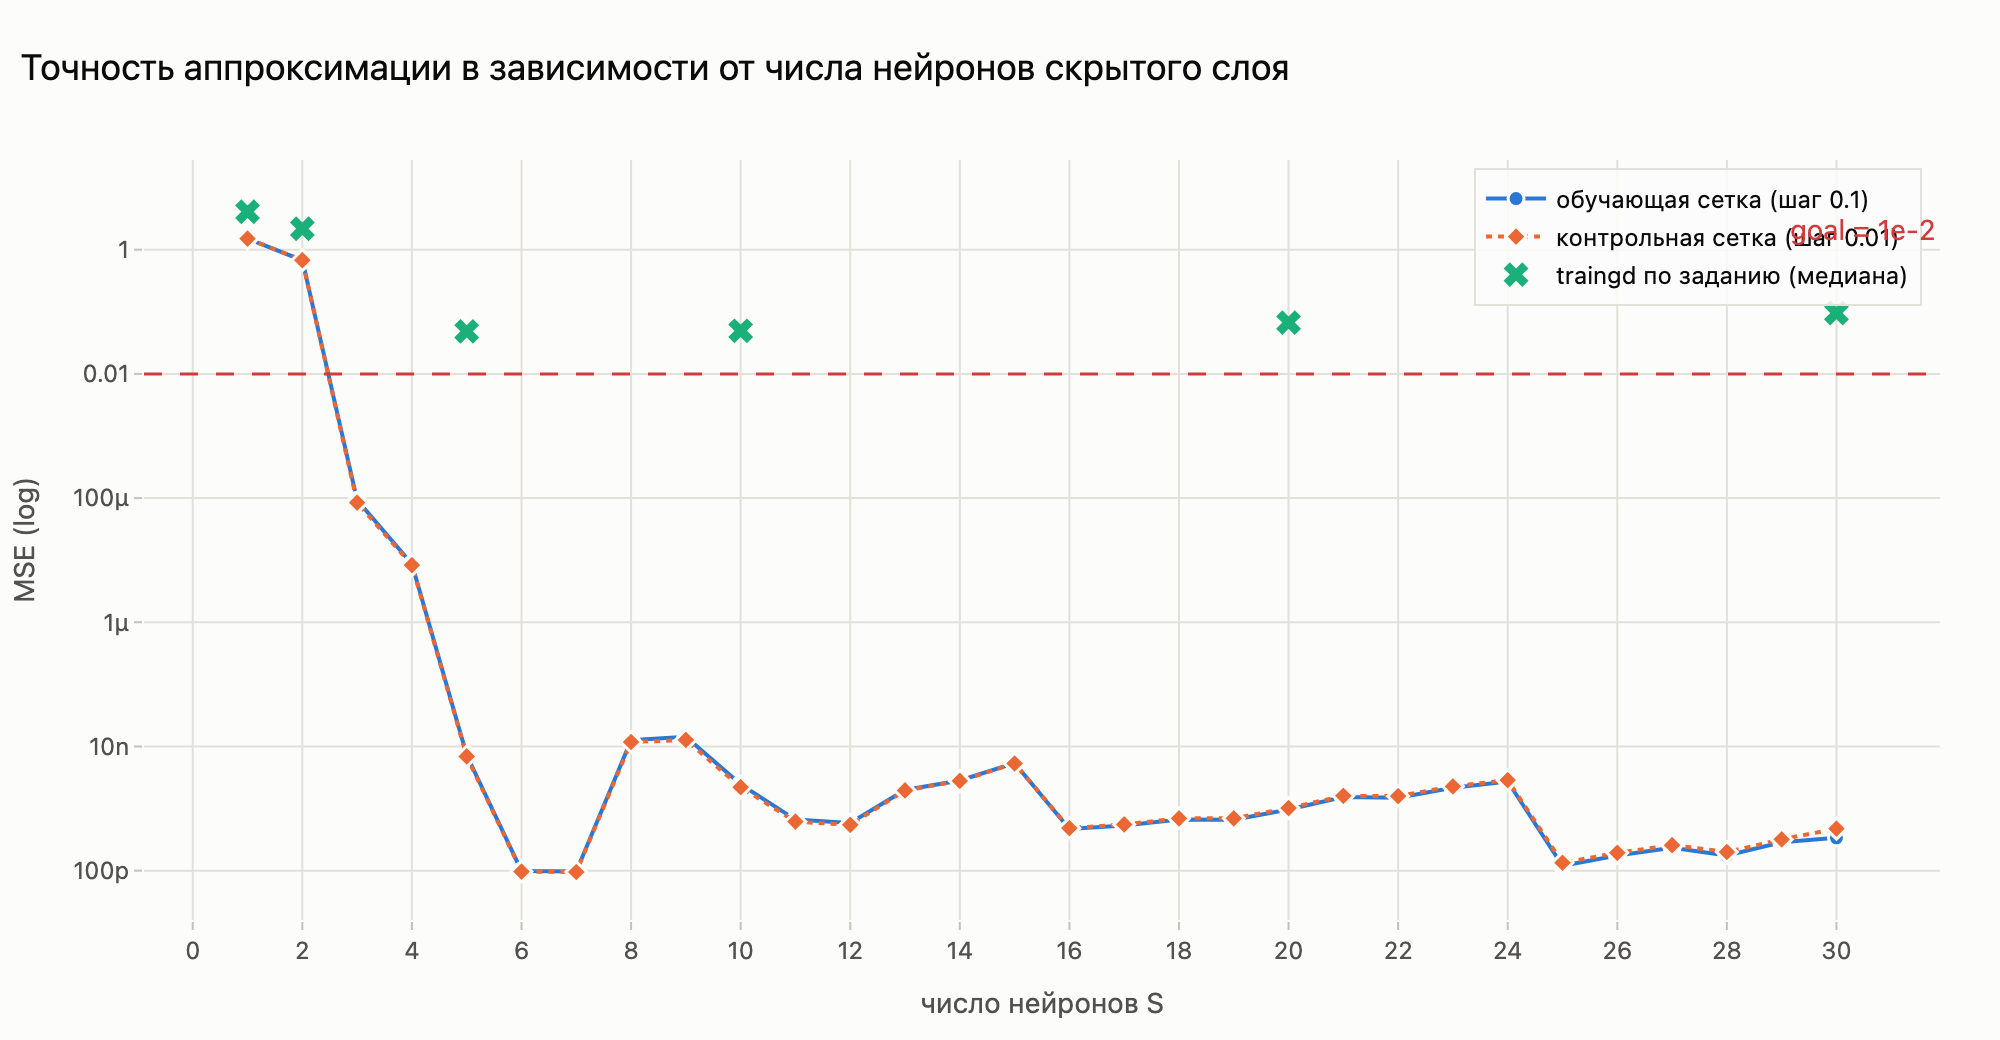
\includegraphics[width=\textwidth]{08_capacity_curve.png}
\caption{Точность аппроксимации в зависимости от числа нейронов скрытого слоя.}
\label{fig:capacity}
\end{figure}

\begin{figure}[H]
\centering
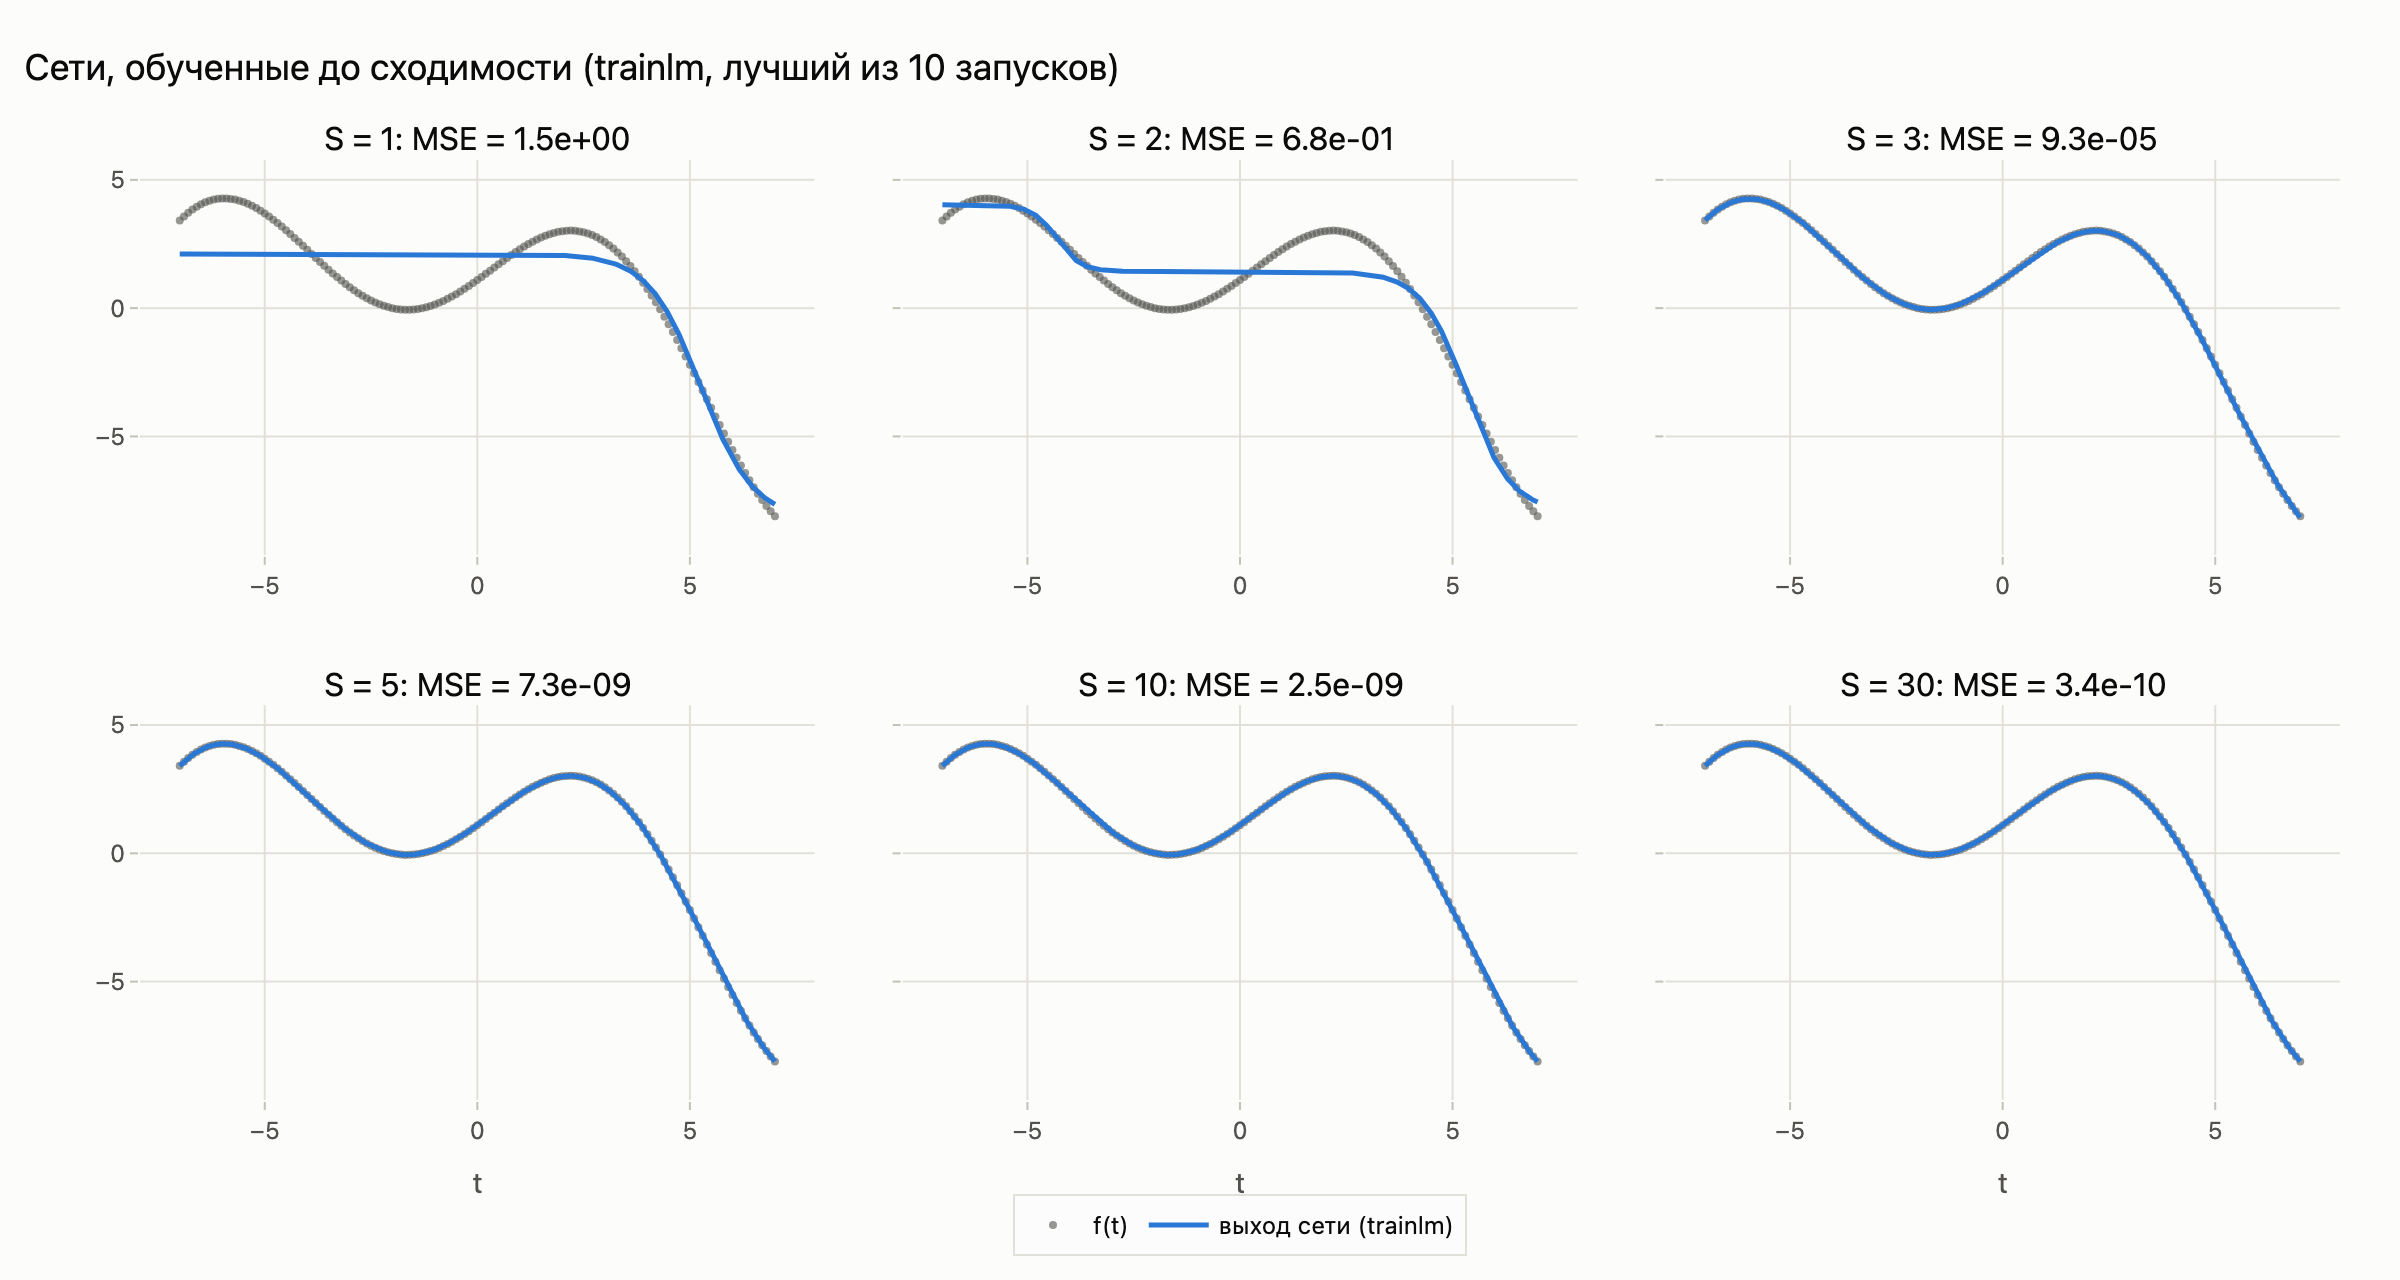
\includegraphics[width=\textwidth]{09_well_trained_models.png}
\caption{Сети, обученные trainlm до сходимости.}
\label{fig:welltrained}
\end{figure}

\begin{figure}[H]
\centering
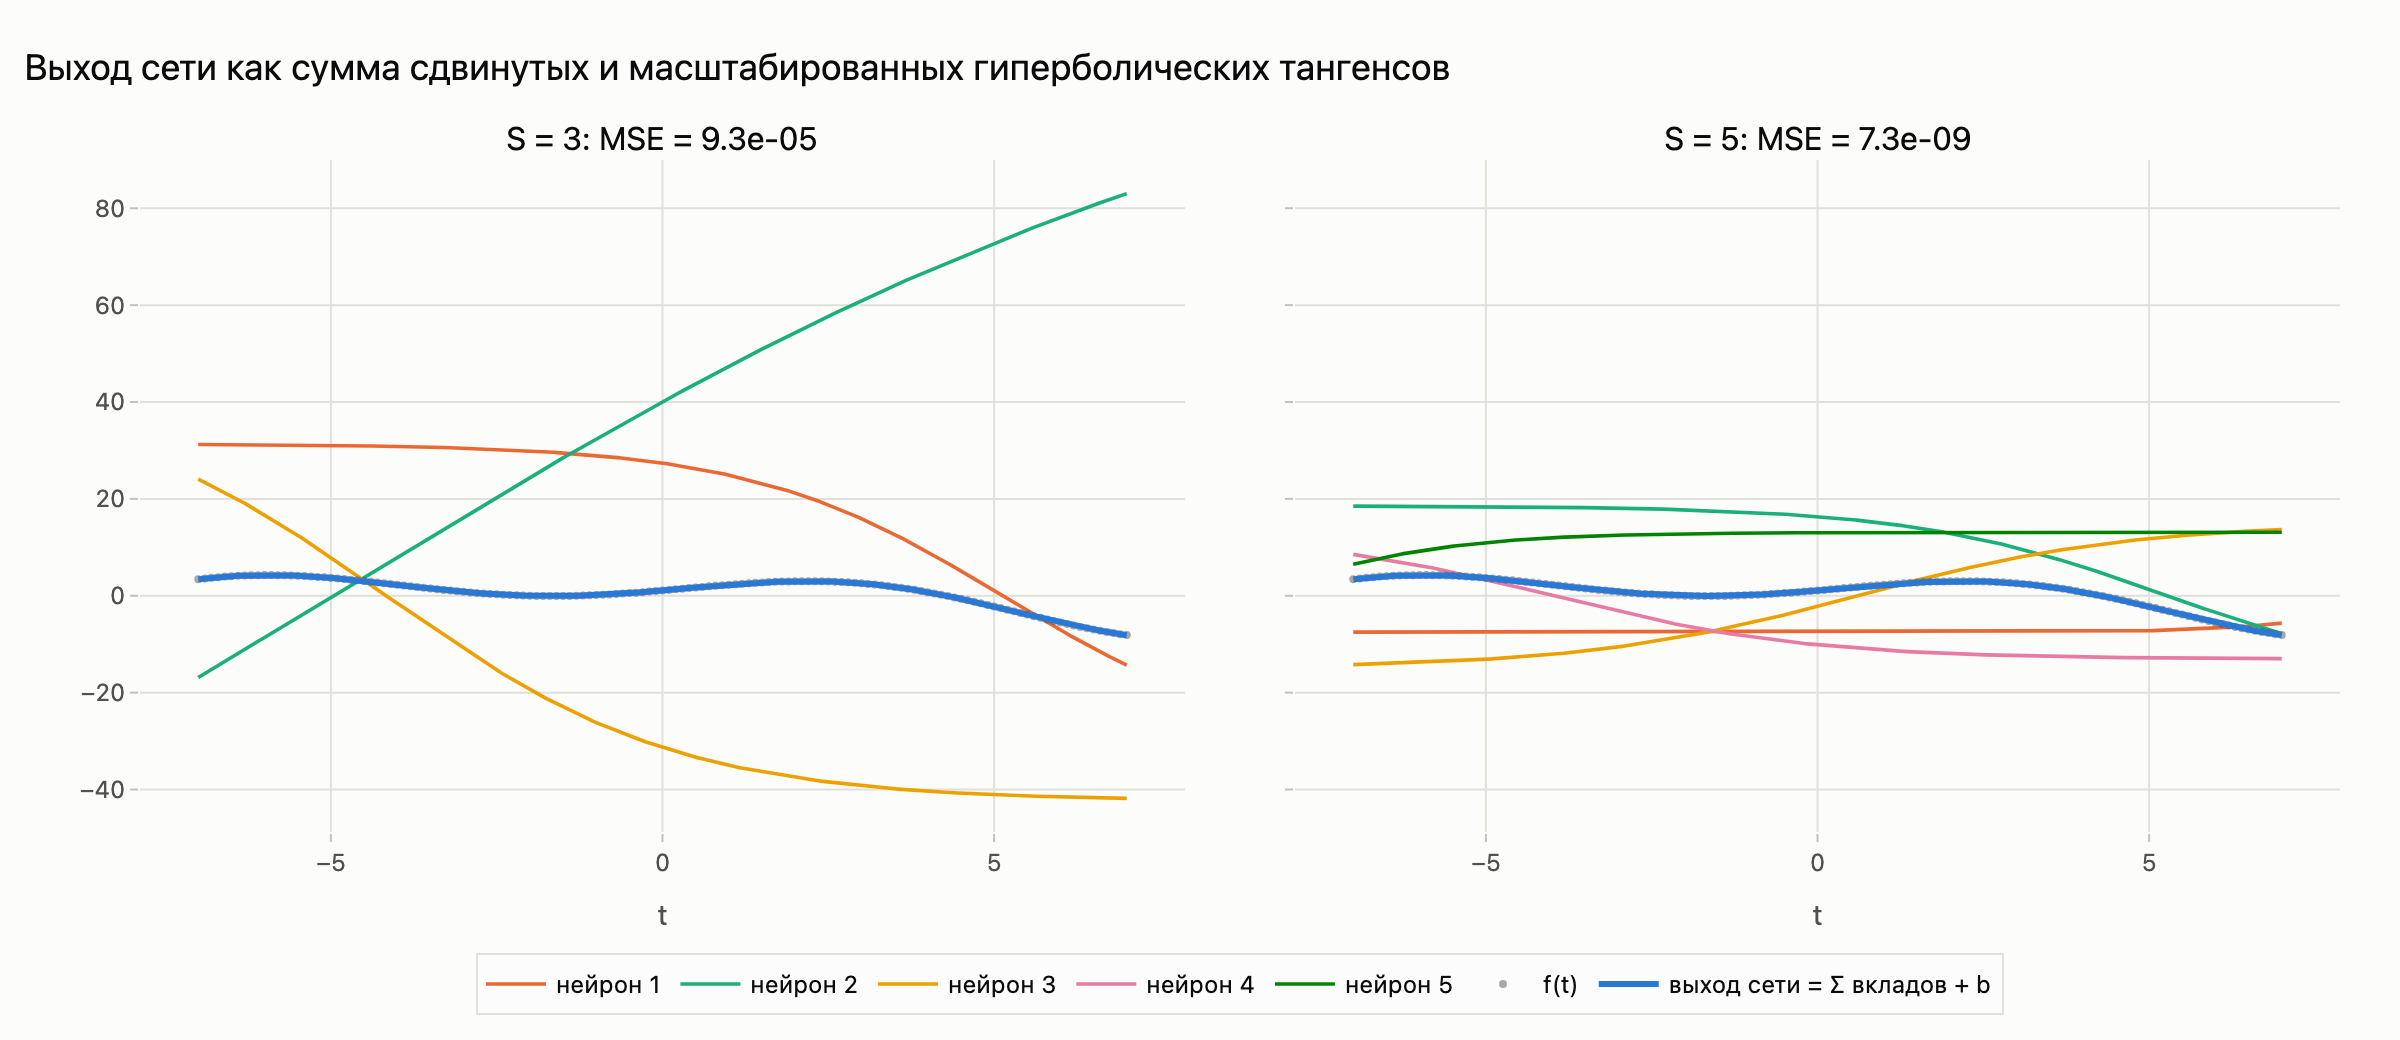
\includegraphics[width=\textwidth]{10_neuron_contributions.png}
\caption{Выход сети как сумма вкладов нейронов скрытого слоя ($S = 3$ и $S = 5$).}
\label{fig:contrib}
\end{figure}

\begin{figure}[H]
\centering
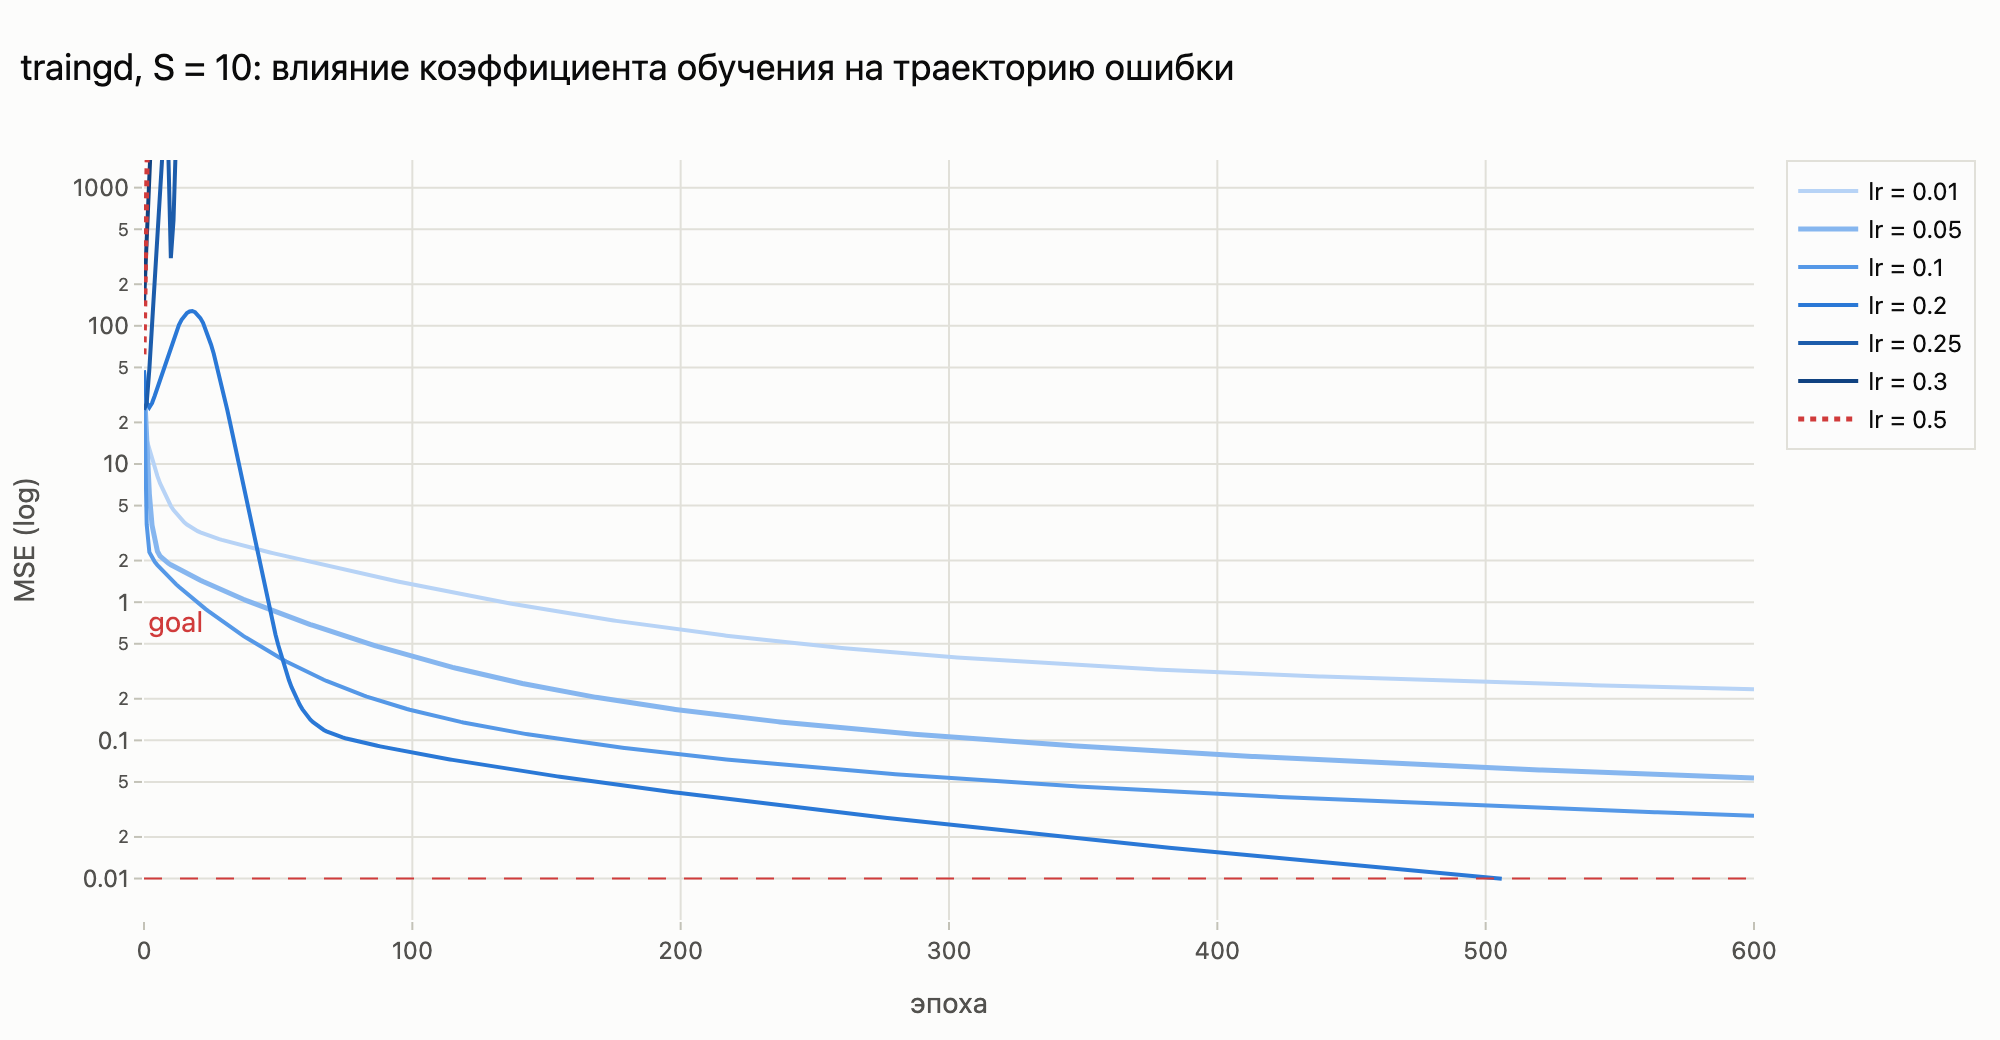
\includegraphics[width=\textwidth]{11_learning_rate.png}
\caption{Влияние коэффициента обучения на траекторию ошибки traingd ($S = 10$).}
\label{fig:lr}
\end{figure}

\begin{figure}[H]
\centering
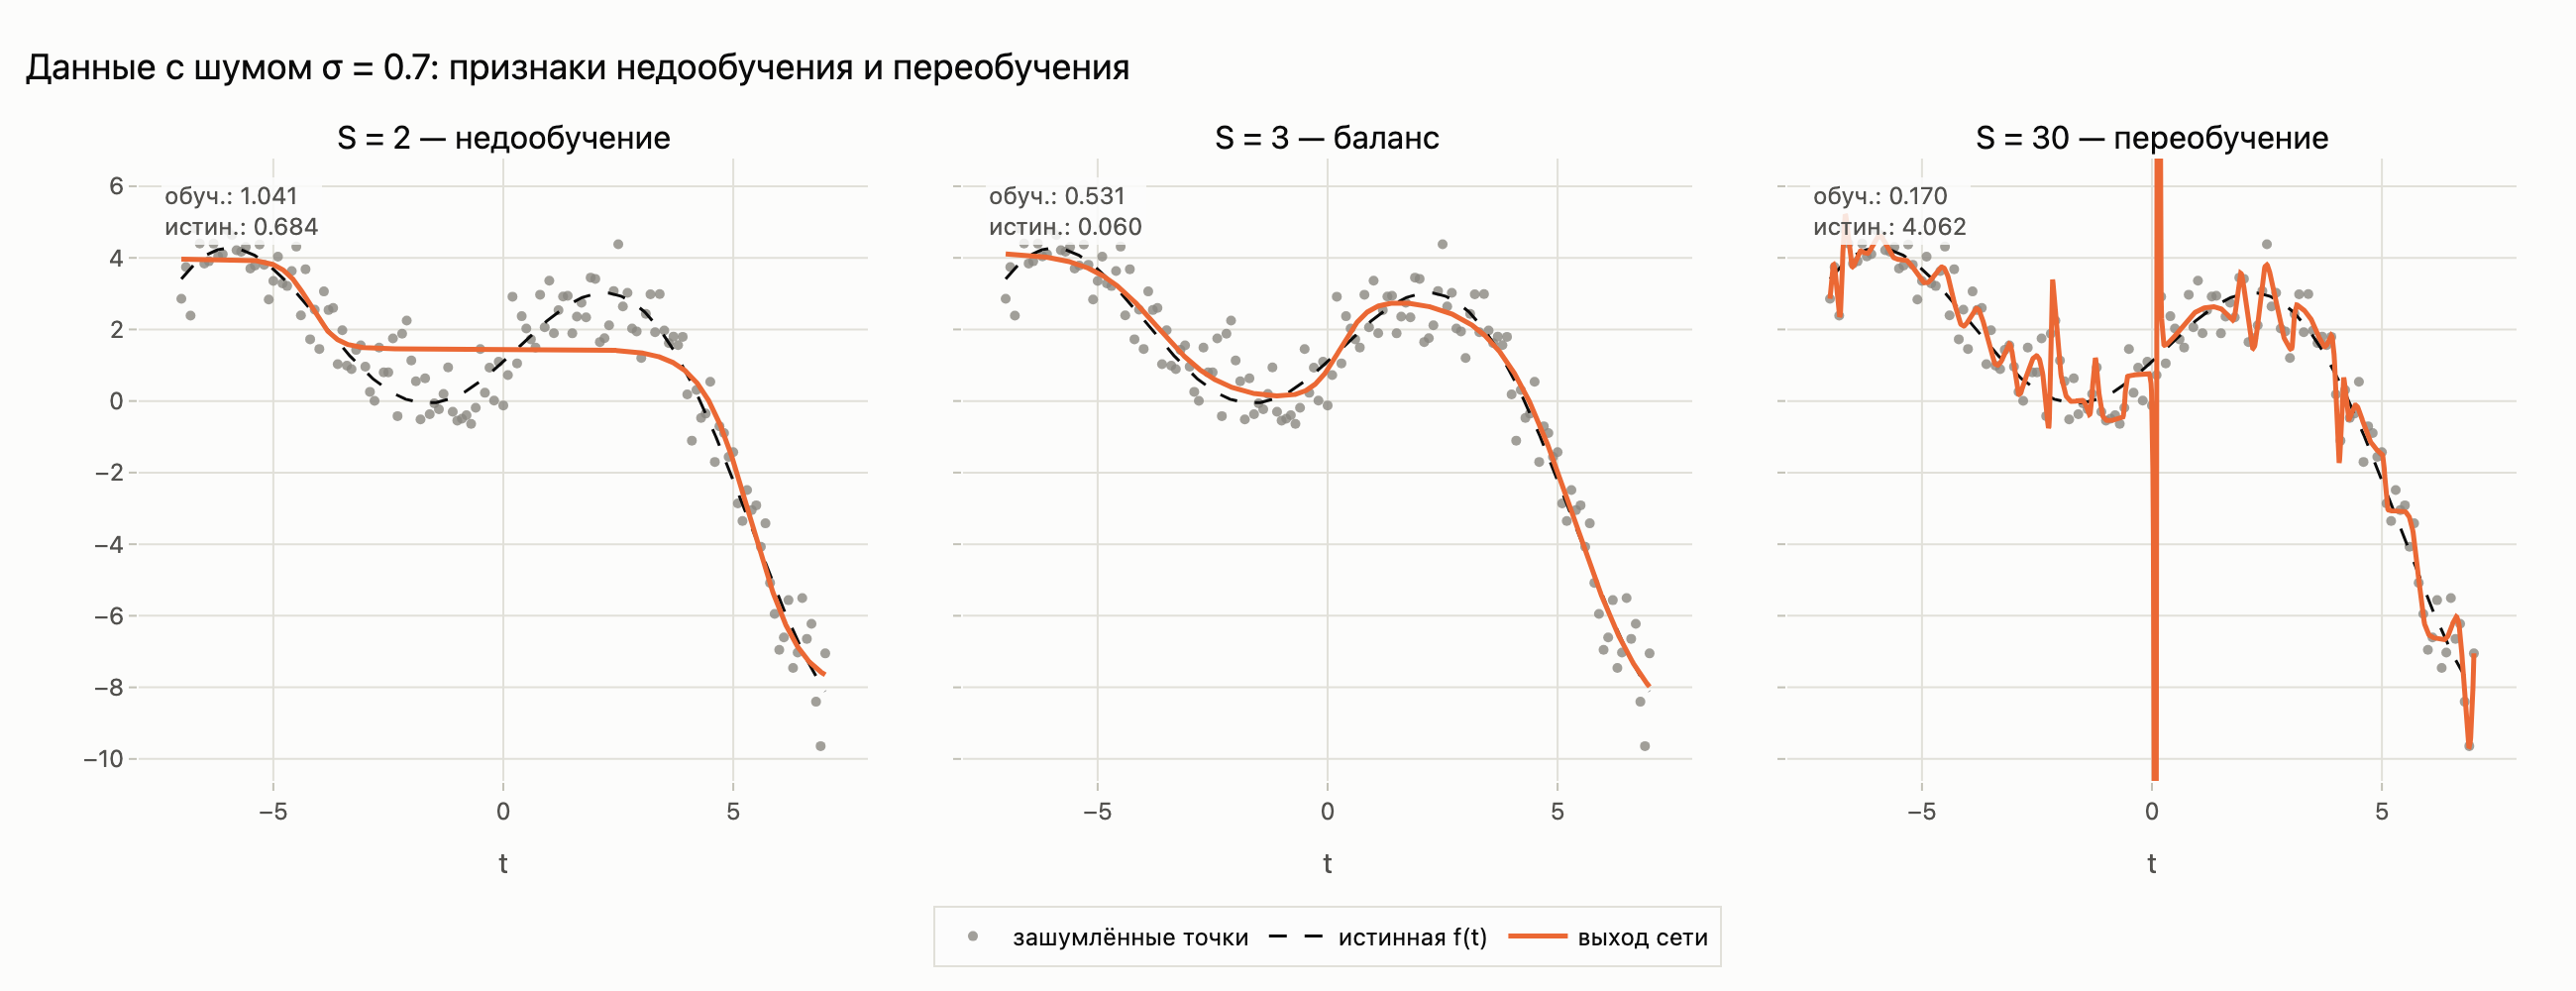
\includegraphics[width=\textwidth]{12_under_overfitting.png}
\caption{Недообучение и переобучение на зашумлённых данных.}
\label{fig:overfit}
\end{figure}

\begin{figure}[H]
\centering
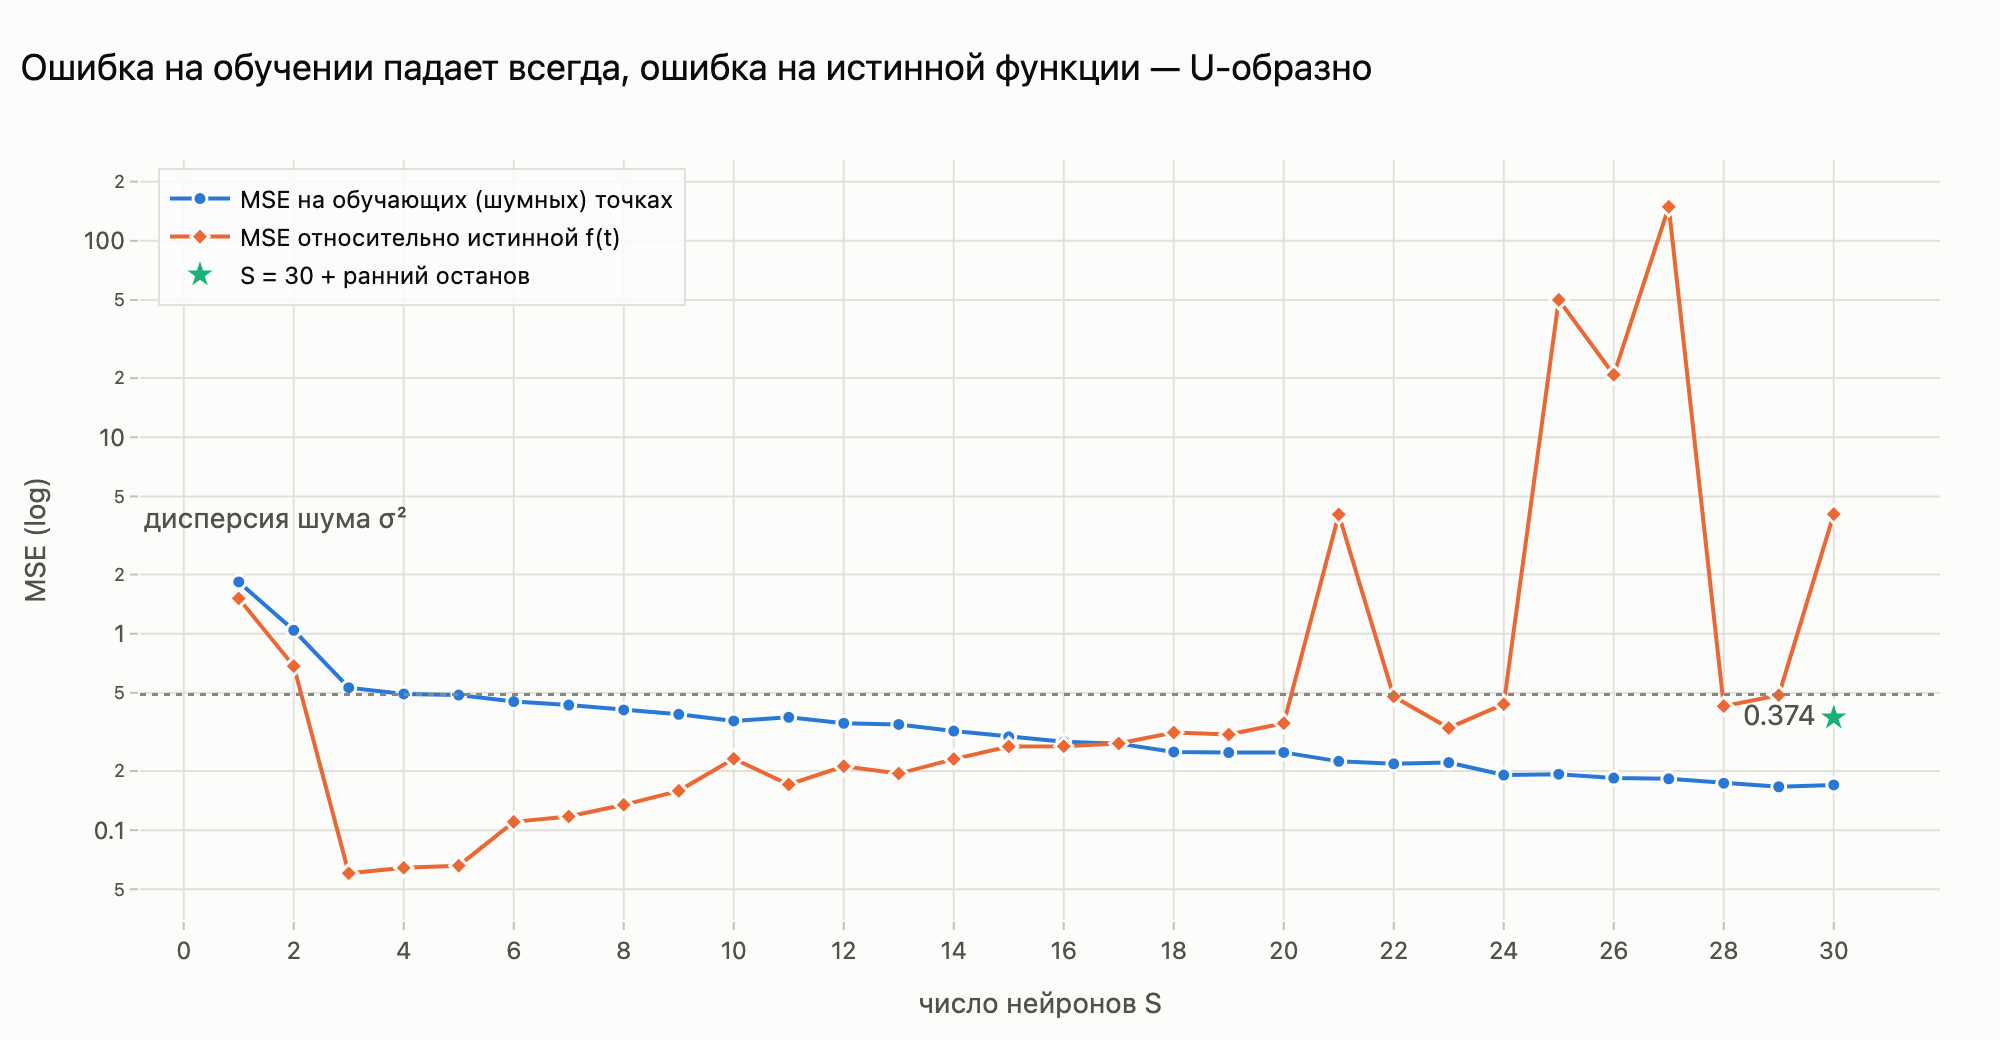
\includegraphics[width=\textwidth]{13_bias_variance.png}
\caption{Ошибка на обучающих точках и относительно истинной функции в зависимости от $S$.}
\label{fig:bv}
\end{figure}

\begin{figure}[H]
\centering
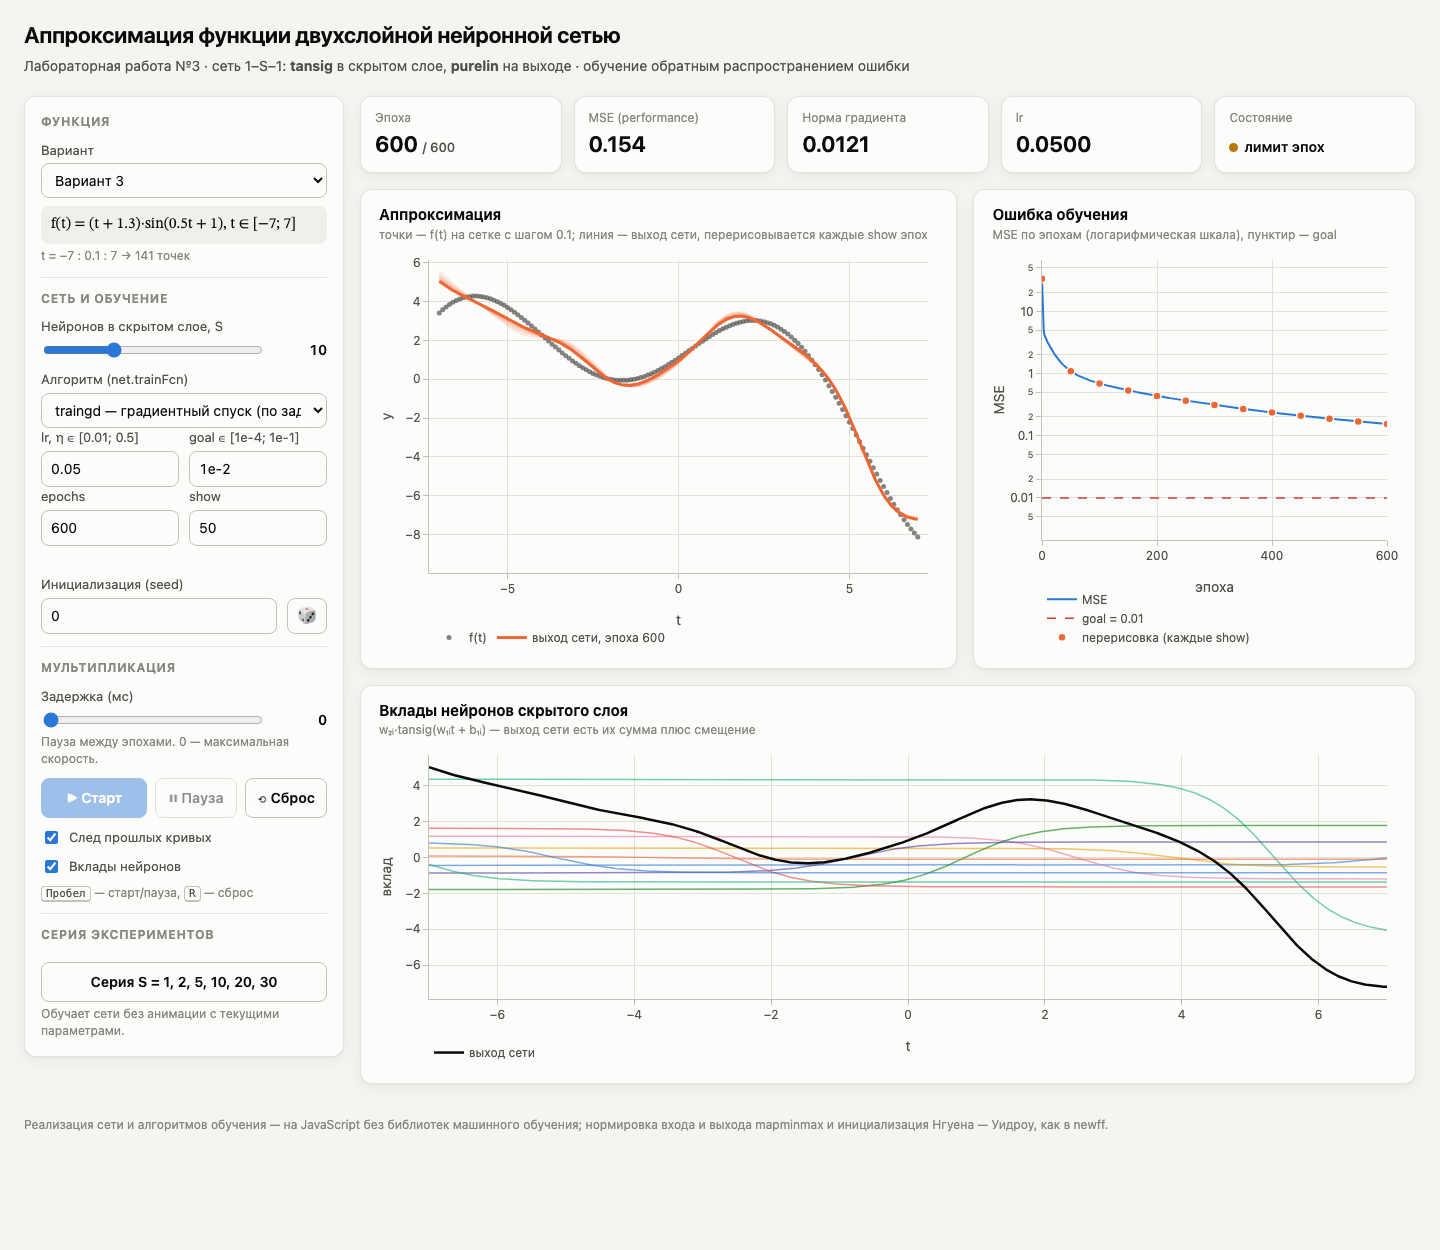
\includegraphics[width=\textwidth]{00_app_screenshot.png}
\caption{Интерактивное приложение \texttt{app/nn\_trainer.html}.}
\label{fig:app}
\end{figure}


\section{Выводы}

В ходе лабораторной работы реализована двухслойная нейронная сеть с сигмоидальным скрытым и линейным выходным слоями, обучаемая методом обратного распространения ошибки, и интерактивное приложение, наглядно показывающее процесс обучения. Экспериментально подтверждена теорема об универсальной аппроксимации: трёх нейронов достаточно, чтобы приблизить функцию варианта~3 с ошибкой $10^{-4}$, пяти~--- с ошибкой $10^{-8}$. Показано, что точность, достигаемая на практике, определяется не только числом нейронов, но и алгоритмом обучения: градиентный спуск с постоянным шагом медленно движется по плохо обусловленной поверхности ошибки и за 600 эпох не достигает цели, тогда как методы с адаптивным шагом и учётом кривизны достигают её за сотни и единицы эпох. Слишком малое число нейронов приводит к недообучению, избыточное на зашумлённых данных~--- к переобучению, которое устраняется уменьшением числа нейронов или ранним остановом по валидационной выборке.

\section{Ответы на контрольные вопросы}

\textbf{1. Какова математическая и алгоритмическая роль нелинейной функции активации в скрытом слое при решении задач аппроксимации?}

Без нелинейности сеть вырождается в линейную модель: $W_2(W_1 t + b_1) + b_2 = W t + b$, поскольку композиция линейных отображений линейна, и при любом числе нейронов получается прямая. Функция \texttt{tansig} превращает каждый нейрон в гладкую <<ступеньку>> $\tanh(w t + b)$ с настраиваемыми положением ($-b/w$), крутизной ($w$) и высотой ($w_2$); выходной слой складывает эти ступеньки, и из их суммы можно собрать кривую любой формы (рисунок~\ref{fig:contrib}). Алгоритмически важно, что \texttt{tansig} дифференцируема, а её производная выражается через уже вычисленное значение: $\tanh'(z) = 1 - \tanh^2 z$, что делает обратное распространение дешёвым. Ограниченность и симметричность относительно нуля улучшают обусловленность обучения.

\textbf{2. Опишите физический и математический смысл алгоритма обратного распространения ошибки (traingd). Как коэффициент обучения (lr) влияет на сходимость траектории?}

Математически \texttt{traingd}~--- градиентный спуск $\theta \leftarrow \theta - \eta\nabla E(\theta)$ по функции MSE. Обратное распространение~--- эффективный способ вычислить градиент по правилу дифференцирования сложной функции: ошибка выхода $\delta_2 = \frac{2}{N}(\hat y - y)$ передаётся назад через веса $W_2$ и умножается на производную активации, $\delta_1 = (\delta_2 W_2)\odot(1 - a_1^2)$; градиент по весу равен произведению сигнала ошибки на вход этого веса. Физически это движение по поверхности ошибки в направлении наискорейшего спуска, при котором каждый вес получает поправку, пропорциональную своему вкладу в ошибку.

Коэффициент \texttt{lr} задаёт длину шага. Малый шаг ($0{,}01$) даёт устойчивую, но очень медленную траекторию (MSE $0{,}23$ за 600 эпох). Увеличение шага ускоряет спуск ($\eta = 0{,}2$~--- цель примерно за 330 эпох), но при $\eta > 2/\lambda_{\max}$ (здесь $\approx 0{,}19$) траектория перескакивает дно <<оврага>>, колеблется с растущей амплитудой и расходится ($\eta \ge 0{,}25$). Поскольку поверхность ошибки сильно вытянута ($\kappa \sim 10^{11}$), один постоянный шаг не подходит одновременно для крутых и пологих направлений~--- отсюда преимущество \texttt{traingdx} и \texttt{trainlm}.

\textbf{3. Сформулируйте суть теоремы об универсальной аппроксимации (теорема Цыбенко / Колмогорова). Что она накладывает на количество слоёв сети?}

Теорема Цыбенко (1989), обобщённая Хорником (1991): для любой непрерывной функции $f$ на компакте $K \subset \mathbb R^n$ и любого $\varepsilon > 0$ существует сеть с \emph{одним} скрытым слоем из конечного числа $S$ сигмоидальных нейронов и линейным выходом, такая что $\max_{x \in K}|f(x) - \hat f(x)| < \varepsilon$. Теорема Колмогорова~--- Арнольда утверждает, что любую непрерывную функцию $n$ переменных можно точно представить суперпозицией непрерывных функций одной переменной и операции сложения. Следствие для архитектуры: двух слоёв (нелинейный скрытый и линейный выходной) \emph{достаточно}, дополнительные слои для самой возможности аппроксимации не нужны. Однако теорема не указывает требуемое число нейронов, не гарантирует, что веса будут найдены градиентным спуском, и ничего не говорит о поведении сети вне обучающих точек. Эксперимент это иллюстрирует: при $S \ge 3$ точность $10^{-2}$ достижима, но \texttt{traingd} за 600 эпох её не находит.

\textbf{4. Каковы явные визуальные признаки недообучения и переобучения (overfitting) сети, наблюдаемые на графике аппроксимации при манипуляциях с размером скрытого слоя?}

\emph{Недообучение} ($S = 1, 2$ или слишком короткое обучение): кривая сети слишком <<жёсткая>>~--- гладкая, с меньшим числом изгибов, чем у функции; экстремумы пропущены ($S = 1$~--- почти наклонная прямая, $S = 2$~--- ступенька); ошибка систематическая, большая и одинаковая на обучающих и контрольных точках.

\emph{Переобучение} ($S = 30$ на зашумлённых данных): кривая проходит почти через каждую обучающую точку, повторяя шум; между точками возникают осцилляции и резкие выбросы (у нас~--- от $-23$ до $+32$ около $t \approx 0{,}1$ при размахе функции около 12); ошибка на обучающих точках ниже уровня шума, а относительно истинной функции многократно выше. Главный признак~--- большой разрыв между ошибками на обучающей и контрольной выборках.

От переобучения следует отличать мелкую рябь у сетей с $S = 20, 30$ после 600 эпох \texttt{traingd}: ошибка на контрольной сетке равна ошибке на обучающей, это недоученность, и она исчезает при продолжении обучения.

\textbf{5. Объясните назначение параметров net.trainParam.show и net.trainParam.goal.}

\texttt{show = 50}~--- период вывода промежуточных результатов: каждые 50 эпох печатается строка протокола (номер эпохи, MSE, норма градиента) и обновляется график; на сам процесс обучения параметр не влияет. В данной работе по нему выполняется перерисовка кривой аппроксимации для мультипликации. \texttt{goal = 1e-2}~--- целевое значение функции качества: обучение прекращается досрочно, как только $E \le$ \texttt{goal}. Это критерий достаточной точности, экономящий эпохи; наряду с ним действуют лимит \texttt{epochs} и порог \texttt{min\_grad}. Слишком малое значение \texttt{goal} на зашумлённых данных толкает сеть к переобучению: ошибки ниже уровня шума можно добиться, только подгоняясь под шум.

\section{Контрольные вопросы для Moodle}

Ниже приведены 30 вопросов в форме, удобной для визуальной проверки. Исходный банк вопросов для загрузки в Moodle сохранен отдельно в файле \texttt{questions.gift.txt}.

\small
\begin{enumerate}[label=\textbf{\arabic*.}, leftmargin=0pt, itemsep=1.2em]
\item Какую архитектуру имеет сеть, используемая в лабораторной работе для аппроксимации функции y = f(t)?
\begin{itemize}[label=$\square$, leftmargin=1.5cm, itemsep=0.2em, topsep=0.3em]
\item Один вход, скрытый слой из S нейронов с tansig и один выходной нейрон с purelin
\item Один вход, два скрытых слоя с purelin и выход с tansig
\item Сеть Кохонена с конкурентным слоем
\item Однослойный персептрон с пороговой функцией активации
\end{itemize}
{\small\textit{Правильный ответ: Один вход, скрытый слой из S нейронов с tansig и один выходной нейрон с purelin.}}

\item Какая функция активации используется в скрытом слое сети?
\begin{itemize}[label=$\square$, leftmargin=1.5cm, itemsep=0.2em, topsep=0.3em]
\item tansig — гиперболический тангенс
\item purelin — линейная функция
\item hardlim — пороговая функция
\item compet — конкурентная функция
\end{itemize}
{\small\textit{Правильный ответ: tansig — гиперболический тангенс.}}

\item Почему в выходном слое сети для аппроксимации используется линейная функция purelin?
\begin{itemize}[label=$\square$, leftmargin=1.5cm, itemsep=0.2em, topsep=0.3em]
\item Потому что выход должен принимать любые вещественные значения, а не только значения из (-1, 1)
\item Потому что линейная функция ускоряет вычисление градиента скрытого слоя
\item Потому что с purelin сеть не может переобучиться
\item Потому что tansig нельзя использовать более одного раза в сети
\end{itemize}
{\small\textit{Правильный ответ: Потому что выход должен принимать любые вещественные значения, а не только значения из (-1, 1).}}

\item Что произойдёт, если в скрытом слое заменить tansig на линейную функцию?
\begin{itemize}[label=$\square$, leftmargin=1.5cm, itemsep=0.2em, topsep=0.3em]
\item Сеть станет эквивалентна линейной модели y = w$\cdot$t + b независимо от числа нейронов
\item Сеть станет точнее аппроксимировать нелинейные функции
\item Обучение перестанет сходиться при любом коэффициенте обучения
\item Число параметров сети уменьшится вдвое
\end{itemize}
{\small\textit{Правильный ответ: Сеть станет эквивалентна линейной модели y = w$\cdot$t + b независимо от числа нейронов.}}

\item Сколько настраиваемых параметров имеет сеть 1–S–1 (один вход, S скрытых нейронов, один выход)?
\begin{itemize}[label=$\square$, leftmargin=1.5cm, itemsep=0.2em, topsep=0.3em]
\item $3S+1$
\item $2S$
\item $S+1$
\item S в квадрате
\end{itemize}
{\small\textit{Правильный ответ: $3S+1$.}}

\item Какая формула задаёт производную функции tanh, используемую в обратном распространении ошибки?
\begin{itemize}[label=$\square$, leftmargin=1.5cm, itemsep=0.2em, topsep=0.3em]
\item 1 $-$ $\tanh^2(z)$
\item $\tanh(z)\cdot$(1 $-$ $\tanh(z)$)
\item $1/(1+e^{-z})$
\item $\tanh(z)$ $-$ 1
\end{itemize}
{\small\textit{Правильный ответ: 1 $-$ $\tanh^2(z)$.}}

\item Что делает алгоритм обучения traingd?
\begin{itemize}[label=$\square$, leftmargin=1.5cm, itemsep=0.2em, topsep=0.3em]
\item Выполняет пакетный градиентный спуск: изменяет веса на $-$lr$\cdot\nabla E$ после каждой эпохи
\item Использует метод Левенберга — Марквардта с адаптивным параметром $\mu$
\item Случайно перебирает веса и сохраняет лучшие
\item Обучает сеть без вычисления градиентов по правилу Хебба
\end{itemize}
{\small\textit{Правильный ответ: Выполняет пакетный градиентный спуск: изменяет веса на $-$lr$\cdot\nabla E$ после каждой эпохи.}}

\item На каком математическом правиле основан алгоритм обратного распространения ошибки?
\begin{itemize}[label=$\square$, leftmargin=1.5cm, itemsep=0.2em, topsep=0.3em]
\item На правиле дифференцирования сложной функции (цепном правиле)
\item На формуле Байеса
\item На методе наименьших модулей
\item На теореме о среднем значении
\end{itemize}
{\small\textit{Правильный ответ: На правиле дифференцирования сложной функции (цепном правиле).}}

\item Какая функция ошибки (performance) минимизируется при обучении сети в лабораторной работе?
\begin{itemize}[label=$\square$, leftmargin=1.5cm, itemsep=0.2em, topsep=0.3em]
\item Среднеквадратичная ошибка MSE
\item Перекрёстная энтропия
\item Максимальная абсолютная ошибка
\item Коэффициент детерминации $R^2$
\end{itemize}
{\small\textit{Правильный ответ: Среднеквадратичная ошибка MSE.}}

\item Что задаёт параметр net.trainParam.show = 50?
\begin{itemize}[label=$\square$, leftmargin=1.5cm, itemsep=0.2em, topsep=0.3em]
\item Период вывода промежуточных результатов и обновления графиков — каждые 50 эпох
\item Количество нейронов скрытого слоя
\item Максимальное число эпох обучения
\item Размер мини-пакета при обучении
\end{itemize}
{\small\textit{Правильный ответ: Период вывода промежуточных результатов и обновления графиков — каждые 50 эпох.}}

\item Что означает параметр net.trainParam.goal = 1e-2?
\begin{itemize}[label=$\square$, leftmargin=1.5cm, itemsep=0.2em, topsep=0.3em]
\item Обучение досрочно прекращается, когда ошибка MSE становится не больше 0.01
\item Коэффициент обучения равен 0.01
\item Веса инициализируются в диапазоне $\pm$0.01
\item Каждая эпоха длится 0.01 секунды
\end{itemize}
{\small\textit{Правильный ответ: Обучение досрочно прекращается, когда ошибка MSE становится не больше 0.01.}}

\item Что задаёт параметр net.trainParam.epochs = 600?
\begin{itemize}[label=$\square$, leftmargin=1.5cm, itemsep=0.2em, topsep=0.3em]
\item Максимальное число эпох (итераций) обучения
\item Число обучающих точек
\item Число нейронов скрытого слоя
\item Количество перезапусков обучения
\end{itemize}
{\small\textit{Правильный ответ: Максимальное число эпох (итераций) обучения.}}

\item Как влияет слишком большой коэффициент обучения lr на градиентный спуск?
\begin{itemize}[label=$\square$, leftmargin=1.5cm, itemsep=0.2em, topsep=0.3em]
\item Траектория перескакивает через минимум, колеблется и может разойтись
\item Обучение становится устойчивее, но медленнее
\item Сеть всегда быстрее достигает глобального минимума
\item Ничего не меняется, так как lr влияет только на вывод графиков
\end{itemize}
{\small\textit{Правильный ответ: Траектория перескакивает через минимум, колеблется и может разойтись.}}

\item Как влияет слишком малый коэффициент обучения lr на градиентный спуск?
\begin{itemize}[label=$\square$, leftmargin=1.5cm, itemsep=0.2em, topsep=0.3em]
\item Обучение устойчиво, но очень медленно, и за отведённые эпохи цель может быть не достигнута
\item Обучение расходится
\item Сеть переобучается уже на первой эпохе
\item Градиенты перестают вычисляться
\end{itemize}
{\small\textit{Правильный ответ: Обучение устойчиво, но очень медленно, и за отведённые эпохи цель может быть не достигнута.}}

\item Какое условие устойчивости градиентного спуска для квадратичной функции ошибки с наибольшим собственным числом гессиана $\lambda_{\max}$?
\begin{itemize}[label=$\square$, leftmargin=1.5cm, itemsep=0.2em, topsep=0.3em]
\item lr $<$ 2 / $\lambda_{\max}$
\item lr $>$ $\lambda_{\max}$
\item lr = $\lambda_{\max}$ / 2
\item lr $<$ 1 / N, где N — число точек
\end{itemize}
{\small\textit{Правильный ответ: lr $<$ 2 / $\lambda_{\max}$.}}

\item Что утверждает теорема об универсальной аппроксимации (Цыбенко, Хорник)?
\begin{itemize}[label=$\square$, leftmargin=1.5cm, itemsep=0.2em, topsep=0.3em]
\item Сеть с одним скрытым слоем с сигмоидальной активацией и достаточным числом нейронов приближает любую непрерывную функцию на компакте с любой точностью
\item Любая сеть с двумя слоями обучается градиентным спуском за конечное число эпох
\item Для аппроксимации функции n переменных нужно не менее n скрытых слоёв
\item Ошибка обучения всегда равна ошибке на новых данных
\end{itemize}
{\small\textit{Правильный ответ: Сеть с одним скрытым слоем с сигмоидальной активацией и достаточным числом нейронов приближает любую непрерывную функцию на компакте с любой точностью.}}

\item Чего НЕ гарантирует теорема об универсальной аппроксимации?
\begin{itemize}[label=$\square$, leftmargin=1.5cm, itemsep=0.2em, topsep=0.3em]
\item Того, что нужные веса будут найдены алгоритмом обучения, и того, сколько нейронов понадобится
\item Существования сети с одним скрытым слоем, приближающей функцию
\item Возможности сколь угодно точного приближения непрерывной функции
\item Применимости к сигмоидальным функциям активации
\end{itemize}
{\small\textit{Правильный ответ: Того, что нужные веса будут найдены алгоритмом обучения, и того, сколько нейронов понадобится.}}

\item Какой вид имеет кривая аппроксимации при недообучении (например, S = 1)?
\begin{itemize}[label=$\square$, leftmargin=1.5cm, itemsep=0.2em, topsep=0.3em]
\item Слишком гладкая и <<жёсткая>>, пропускает экстремумы функции; ошибка велика и на обучающих, и на новых точках
\item Проходит через каждую обучающую точку и сильно колеблется между ними
\item Совпадает с функцией на обучающих точках, но расходится только вне отрезка
\item Всегда является горизонтальной прямой y = 0
\end{itemize}
{\small\textit{Правильный ответ: Слишком гладкая и <<жёсткая>>, пропускает экстремумы функции; ошибка велика и на обучающих, и на новых точках.}}

\item Какой визуальный признак переобучения сети?
\begin{itemize}[label=$\square$, leftmargin=1.5cm, itemsep=0.2em, topsep=0.3em]
\item Кривая повторяет шум обучающих точек и осциллирует между ними; ошибка на обучении мала, на контрольных точках велика
\item Кривая проходит ниже всех обучающих точек
\item Кривая монотонна на всём отрезке
\item Ошибка одинаково велика на обучающих и контрольных точках
\end{itemize}
{\small\textit{Правильный ответ: Кривая повторяет шум обучающих точек и осциллирует между ними; ошибка на обучении мала, на контрольных точках велика.}}

\item Как в общем случае меняются ошибка на обучающих данных и ошибка на новых данных при росте числа нейронов S на зашумлённой выборке?
\begin{itemize}[label=$\square$, leftmargin=1.5cm, itemsep=0.2em, topsep=0.3em]
\item Ошибка на обучении уменьшается, а ошибка на новых данных сначала падает, затем растёт (U-образно)
\item Обе ошибки монотонно растут
\item Обе ошибки монотонно убывают до нуля
\item Ошибка на обучении растёт, а на новых данных убывает
\end{itemize}
{\small\textit{Правильный ответ: Ошибка на обучении уменьшается, а ошибка на новых данных сначала падает, затем растёт (U-образно).}}

\item Как узнать, что мелкая <<рябь>> на кривой после короткого обучения большой сети — это недоученность, а не переобучение?
\begin{itemize}[label=$\square$, leftmargin=1.5cm, itemsep=0.2em, topsep=0.3em]
\item Ошибка на контрольных точках между узлами практически равна ошибке на обучающих точках и уменьшается при продолжении обучения
\item Рябь всегда означает переобучение
\item Нужно уменьшить число обучающих точек
\item Достаточно посмотреть на значение параметра show
\end{itemize}
{\small\textit{Правильный ответ: Ошибка на контрольных точках между узлами практически равна ошибке на обучающих точках и уменьшается при продолжении обучения.}}

\item Зачем в newff входы и цели по умолчанию нормируются функцией mapminmax?
\begin{itemize}[label=$\square$, leftmargin=1.5cm, itemsep=0.2em, topsep=0.3em]
\item Чтобы привести данные к диапазону [-1, 1], где tansig не насыщается и градиенты хорошо обусловлены
\item Чтобы уменьшить число эпох до одной
\item Чтобы сеть могла работать без скрытого слоя
\item Чтобы исключить из выборки выбросы
\end{itemize}
{\small\textit{Правильный ответ: Чтобы привести данные к диапазону [-1, 1], где tansig не насыщается и градиенты хорошо обусловлены.}}

\item В чём идея инициализации Нгуена — Уидроу (initnw)?
\begin{itemize}[label=$\square$, leftmargin=1.5cm, itemsep=0.2em, topsep=0.3em]
\item Распределить активные области сигмоид скрытых нейронов равномерно по диапазону входа
\item Инициализировать все веса нулями
\item Задать всем нейронам одинаковые веса и смещения
\item Выбрать веса так, чтобы сеть сразу была линейной
\end{itemize}
{\small\textit{Правильный ответ: Распределить активные области сигмоид скрытых нейронов равномерно по диапазону входа.}}

\item Почему нельзя инициализировать все веса скрытого слоя одинаковыми значениями?
\begin{itemize}[label=$\square$, leftmargin=1.5cm, itemsep=0.2em, topsep=0.3em]
\item Все нейроны получат одинаковые градиенты и останутся одинаковыми — сеть фактически будет иметь один нейрон
\item Потому что сеть сразу переобучится
\item Потому что MSE станет отрицательной
\item Потому что тогда нельзя вычислить выход purelin
\end{itemize}
{\small\textit{Правильный ответ: Все нейроны получат одинаковые градиенты и останутся одинаковыми — сеть фактически будет иметь один нейрон.}}

\item Чем алгоритм traingdx отличается от traingd?
\begin{itemize}[label=$\square$, leftmargin=1.5cm, itemsep=0.2em, topsep=0.3em]
\item Использует момент и адаптивно меняет коэффициент обучения в зависимости от изменения ошибки
\item Использует матрицу Якоби и решает систему линейных уравнений
\item Обучает только выходной слой
\item Не использует градиент ошибки
\end{itemize}
{\small\textit{Правильный ответ: Использует момент и адаптивно меняет коэффициент обучения в зависимости от изменения ошибки.}}

\item Почему метод Левенберга — Марквардта (trainlm) сходится за единицы эпох там, где traingd требует тысячи?
\begin{itemize}[label=$\square$, leftmargin=1.5cm, itemsep=0.2em, topsep=0.3em]
\item Он учитывает кривизну поверхности ошибки через приближение гессиана $J^{\top}J$ и делает шаг, близкий к ньютоновскому
\item Он использует больший фиксированный коэффициент обучения
\item Он пропускает вычисление ошибки на каждой эпохе
\item Он уменьшает число параметров сети
\end{itemize}
{\small\textit{Правильный ответ: Он учитывает кривизну поверхности ошибки через приближение гессиана $J^{\top}J$ и делает шаг, близкий к ньютоновскому.}}

\item Что показывает мультипликация процесса обучения — перерисовка кривой аппроксимации каждые show эпох?
\begin{itemize}[label=$\square$, leftmargin=1.5cm, itemsep=0.2em, topsep=0.3em]
\item Как кривая сети постепенно <<изгибается>> и подстраивается под форму эталонной функции по мере уменьшения ошибки
\item Как меняется число нейронов в скрытом слое
\item Как меняется исходная функция f(t)
\item Как сеть выбирает шаг дискретизации t
\end{itemize}
{\small\textit{Правильный ответ: Как кривая сети постепенно <<изгибается>> и подстраивается под форму эталонной функции по мере уменьшения ошибки.}}

\item Как формируется выход двухслойной сети с tansig и purelin?
\begin{itemize}[label=$\square$, leftmargin=1.5cm, itemsep=0.2em, topsep=0.3em]
\item Как взвешенная сумма сдвинутых и масштабированных гиперболических тангенсов плюс смещение
\item Как произведение выходов всех скрытых нейронов
\item Как максимум из выходов скрытых нейронов
\item Как выход одного случайно выбранного нейрона
\end{itemize}
{\small\textit{Правильный ответ: Как взвешенная сумма сдвинутых и масштабированных гиперболических тангенсов плюс смещение.}}

\item Что помогает бороться с переобучением сети на зашумлённых данных?
\begin{itemize}[label=$\square$, leftmargin=1.5cm, itemsep=0.2em, topsep=0.3em]
\item Ранний останов по валидационной выборке, уменьшение числа нейронов или регуляризация
\item Увеличение числа нейронов до максимума
\item Уменьшение целевой ошибки goal до нуля
\item Отказ от контрольной выборки
\end{itemize}
{\small\textit{Правильный ответ: Ранний останов по валидационной выборке, уменьшение числа нейронов или регуляризация.}}

\item Зачем при исследовании влияния числа нейронов повторять обучение с разными начальными весами?
\begin{itemize}[label=$\square$, leftmargin=1.5cm, itemsep=0.2em, topsep=0.3em]
\item Потому что результат градиентного спуска зависит от инициализации, и один запуск может оказаться случайно удачным или неудачным
\item Потому что при одном запуске сеть не может вычислить градиент
\item Потому что каждое новое обучение увеличивает число нейронов
\item Потому что так требует функция mapminmax
\end{itemize}
{\small\textit{Правильный ответ: Потому что результат градиентного спуска зависит от инициализации, и один запуск может оказаться случайно удачным или неудачным.}}

\end{enumerate}



\end{document}
